\documentclass[11pt,letterpaper]{book}
\usepackage{emptypage}
\usepackage{pdflscape}
% math stuffs
\usepackage{mathtools}
%\usepackage{wasysym}
\usepackage{seqsplit}
\usepackage{multirow}

% fontenc for the accents and junk
\usepackage[utf8]{luainputenc}
\usepackage[T1]{fontenc}

% Typeface
%\usepackage[adobe-utopia]{mathdesign}
%\usepackage{fourier}
%\usepackage{fouriernc}
%\usepackage{mathptmx}
%\usepackage{tgtermes}
%\usepackage{pxfonts}
%\usepackage{newpxtext,newpxmath}
%\usepackage[sc]{mathpazo}
%\usepackage[oldstylenums]{kpfonts}
\usepackage{kpfonts}
%\usepackage{tgpagella}
%\usepackage[garamond]{mathdesign}
%\usepackage{garamondx}
%\usepackage{ebgaramond}

% Need Greek character support
\usepackage{textgreek}

% Umm
\usepackage{adjustbox}
\usepackage{multirow}
\usepackage{verbatimbox}
\usepackage{caption}
\usepackage{ftnxtra}
\usepackage{longtable}
\usepackage[rightmargin=0.0pt,indentfirst=false]{quoting}

% Makes graphics easy
\usepackage{graphicx}

\usepackage{titling}

\usepackage{perpage} %the perpage package
\MakePerPage{footnote} %the perpage package command

% PDF is always pretty
\DeclareGraphicsExtensions{.pdf}

% Line spacing, 1.4 is pretty but YMMV
\linespread{1.4}

% Homespun macros 
%\newcommand{\wlt}[1]{{\Large\;\textless\normalsize}#1{\Large\textgreater\;\normalsize}}
%\newcommand{\wlc}[1]{{\large\;\{\normalsize}#1{\large\}\;\normalsize}}
%\renewcommand{\arraystretch}{0.7}
\newcommand{\Hair}{\ifmmode\mskip1mu\else\kern0.12em\fi}

\renewcommand{\thefootnote}{\fnsymbol{footnote}}

\begin{document}

\frontmatter

\setlength{\droptitle}{-96pt}

\pretitle{\begin{flushleft}}
\title{\Huge{\textsc{The True Squaring of the Circle and the Hyperbola}} \\
\vskip 1.0em \Large{In its own species of proportion, \\
Discovered and proved.}}
\posttitle{\par\end{flushleft}\vskip 4.5em}

\preauthor{\begin{flushleft}}
\author{\LARGE{James Gregory} \\
\Large{Translation from the Latin by Walter Jacob}\vskip 10.0em}
\postauthor{\end{flushleft}}

\predate{\begin{tabular}{p{140pt} p{100pt}} &\raggedleft}
\date{1667 \\ Aberdeen, Scottland}
\postdate{\end{tabular}}

\maketitle

\chapter*{\Huge\textnormal{\textsc{Welcome,}} \\ \textnormal{\textsc{Reader
of Geometry}}}

I was contemplating at length, dear Reader, whether analysis with its many
operations, and the general method of investigating all proportions of a
quantity, are sufficient, as Descartes claims at the beginning in his Geometry.
If it were indeed so, it could be that it is possible to use it to demonstrate
the oft-sung feat of squaring of the circle. Whenever I turn this over in my mind I
readily see from the discoveries made so far on the properties of the circle
that no one can establish such a result by use of analysis. Thus it occurred to
me to search out the method that follows, first by considering the common 
circle. In doing so I hit upon the convergent sequence of polygons, the limit of
which is the circular sector. I saw here at once a trace of analysis. It
followed that the convergent series applies naturally not only in the case of
the circle, but likewise in more general consideration. Thus from the
properties of the circle followed the cases of ellipse and the hyperbola with no
effort, and thus the infallible quadrature of every conic section was revealed
to me. However the convergent series of polygons soon turned the tables on me,
and I was forced to ply all of my arts to the insuperable difficulty of
discovering its limit. By pondering its very nature, I saw that the purpose of
analysis as well as of common algebra is not only to
resolve problems, but likewise to demonstrate their impossibility (when its
useful). After this first difficulty was put to rest, I also conquered the
more general case, as I claim above. Indeed I uncovered the true and legitimate
quadrature, in its own species of proportion, not only of the circle (which I
had set out to do at the beginning) but of all of the conic sections, and I revealed
an entire species of proportion previously unknown to the field of Geometry.
I can calculate this proportion as closely as needed in relation to the
dimension of the conic section, and can easily demonstrate the very rapid
extraction of square roots of solid surds (unless I am very much mistaken). In
fact, such approximations apply mathematically to every incommensurable
proportion, such that we might better understand the nature of the proportion. I
might speak of a proportion insofar as it is derived by some analytic
operations (i.e.\ of the common arithmetic), and the proportion is then known to
us in numbers or in the continuation of some discrete quantities. I am not
afraid to render these operations geometrically in the style of Decartes.

First note that we always know how to relate commensurable quantities, or
those having a common number between them. We cannot perceive incommensurable
proportions unless they themselves are relatively commensurable, for the
infinitude renders us ignorant, blunting our minds and impeding our simple
notions. Two of the five arithmetic operations, addition and subtraction, are
the most elementary. Multiplication is composed of addition, division from
subtraction. Square root extraction, which in general is nothing more than
finding commensurable proportions, and which closely approaches an analytically
incommensurable proportion, is composed from the aforementioned four. Our sixth
operation, which in general is nothing more than finding commensurable
proportions closely approximating a non-analytic proportion, is composed of the
previous five. It will be noted that just as no fractional numbers are produced
from integers by addition, subtraction or multiplication, but only by division,
and just as no incommensurable numbers are produced from commensurables by
addition subtraction, multiplication or division, but only by square root
extraction, so non-analytic quantities are not born from analytic numbers by
addition, subtraction, multiplication, division, or square root extraction, but
rather from this sixth operation. As such this new operation of ours may be
added to arithmetic and a new species of ratio may be added to geometry, which
(as I demonstrate in this treatise) allows us to understand the analyticity of
the ratio of the circle to the square of its diameter as a kind of ratio we
currently know how to produce, just as square root extraction allows us to
understand the ratio between the side of the square and its diameter in terms of
commensurability.

It seems clear to me that the whole of the proof cannot be reduced to
gemometric language, for in order to accomplish this we would use no small
number of analytic magnitudes that are mutually related and
incommensurable in kind.  I am amazed that this idea has never been written
about, as it opens wide the plains of discovery.
For from this approach comes proof that the mesolabe\footnote{An
apparatus of Eratosthenes used to construct $n$th roots.} cannot be achieved by
the power of the straightedge and compass, likewise that not always can
affected equations be reduced to pure ones\footnote{Pure equations contain
only one term raised to a power, as with $x^7 = c$.  Affected equations contain
multiple such terms, as with $x^9-ax^b+x = c$.}, 
%\emph{or similarly that it be made necessary to
%the minumum of such a class of curve to the mechanical solution of such
%equations with such an innumerable quantity:} 
or such similar
things which even by the most outstanding mathematicians are impossible to show
by means of analysis, and are sought in vain daily by the uninititated.
Euclid dedicated the entirety of his tenth book (except for a few minor general
propositions) on incommensurables produced from the extraction of square roots.
I don't know to what extent this material is covered in any other treatise,
although it be not only very useful to speculative geometry but is also an
extremely remarkable theory in its own right.
For example, in a geometric progression in which the first term is given by a
commensurable length or a power of such, and the second is any
other whichever, be it binomial, trinomial, etc., it is impossible that the
sequences progressing infinitely from these two terms will be mutually
commensurable by a length or a power of such.
I have more to offer, but perhaps I shall reserve this for a more favorable
time.
It is enough for the timebeing that this matter has been proven analytically.
And if indeed analysis agreeing to such a glaring degree isn't compelling
enough, there is the geometry, neither refuting nor being refuted by
analysis, which in the past was proved by geometry.
From this invention I deduce some new angular sections and a doctrine of
logarithms, some easy, most expeditious in practice and fortified by geometric
demonstration.
As far as the legnthy construction of logarithms is concerned, a more preferable
conjecture is seen than what is known, as well as the division of an angle into
more than five equal parts.
Counting by prime numbers can be done only with great difficulty.
I demonstrate all of these sums (or those that I can) quickly and clearly.
And I am not careful in citations, in so far as foreign books of such work are
lacking, and indeed I suppose you are not poorly versed in geometry,
otherwise you will acquire no fruit by your labor.
It remains for me to warn you that I always aspire to the demonstration of
utmost generality, not only in this but also in my other works.
%Thus as I admire R. P. Francis Eschinard from the Society of Jesus in his
% optical dialog on page 26 to confirm to have proved to me in my optica promota, that image is seen in the same angle from the vertex of emersion as visible from the incident vertex, not only in elliptic and hyperbolic lenses, but also in all of my particular theory from which the whole of optical science is deduced, namely pages 26-27, 44-47, and 50.

\ldots

\mainmatter
\begin{center}
\Huge\textsc{Definitions.}
\end{center}
\begin{enumerate}
  \item Let two lines be drawn from the center of a circle, ellipse, or
  hyperbola to its perimeter. We call the piece bound by those two lines and
  the segment of the perimeter a sector.
  
  \item Let the segment of the perimeter between the two lines be subtended
  any number of times, forming rectilinear triangles (where the common vertex
  is the center of the conic section and the bases are the subtending lines).
  Then if the conic section is a circle or ellipse we call the figure created
  by combining these triangles a regular inscribed triangle, if it is a
  hyperbola then we call the figure a regular circumscribed polygon.
  
  \item Let the segment of the perimeter between the lines be made tangent to
  lines any number of times and let lines be drawn from the tangents to the
  center of the conic section, and further require that each of the
  quadrilaterals, understood as being composed from successive tangent lines
  and the lines to the center, be equal. If the conic section is a circle or an
  ellipse, then I call the figure created by the combination of these a regular
  circumscribed polygon. If it is a hyperbola then I call it a regular
  inscribed polygon.
  
  \item Let all of the vertices of the subtending angles (except those to the
  center of the conic section) of the regular polygon touch all of the points
  of contact of the regular polygon with the tangents. I call this a complex
  polygon.
  
  \item We say a magnitude is composed of magnitudes, when one magnitude
  makes other magnitudes by addition, subtraction, multiplication, division,
  root extraction, or any other operation imaginable.
  
  \item When a magnitude is composed of magnitudes by addition, subtraction,
  multiplication, division, or root extraction, we say it is composed
  analytically.
  
  \item When magnitudes can be composed analytically of magnitudes which are
  mutually commensurable, we say they are mutually analytic.
  
  \item Let the magnitude $X$ be composed of some magnitudes $A$, $B$, $C$, $D$,
  and $E$, and the magnitude $Z$ be composed of magnitudes $F$, $G$, $C$, $D$,
  and $E$ by the same method and operations as $X$ only with the magnitudes $F$
  and $G$ in place of $A$ and $B$. If this is so, then we say that the magnitude
  $X$ is composed of $A$ and $B$ by the same method as $Z$ is composed of $F$
  and $G$.
  
  \item Let there be two magnitudes $A$ and $B$ of which are composed two other
  magnitudes $C$ and $D$, whose the difference is less than that of $A$ and $B$.
  Also let $E$ be composed from $C$ and $D$ by the same method as $C$ is
  composed of $A$ and $B$, and $F$ be composed from $C$ and $D$ by the same
  method as $D$ is composed of $A$ and $B$. And further still let $G$ be
  composed from $E$ and $F$ by the same method as $E$ is composed of $C$ and $D$
  and $C$ is composed by $A$ and $B$, and let $H$ be composed from $E$ and $F$
  by the same method as $F$ is composed of $C$ and $D$ and $C$ is composed by
  $A$ and $B$. Continue thus. I call this a convergent series.
  
  \item Terms being placed next to each other as $A$ and $B$, or $C$ and $D$,
  or $E$ and $F$, or $G$ and $H$, are called convergent terms.
\end{enumerate}

\begin{center}
\Large\textsc{Assumptions.}
\end{center}
\begin{enumerate}
  \item We assume that magnitudes composed of given mutually analytic
  magnitudes be mutually analytic themselves as well as analytic with the given
  magnitudes.
  
  \item Likewise we assume that magnitudes that cannot be analytically
  composed from given mutually analytic magnitudes not be analytic with the
  given magnitudes.
\end{enumerate}
The preceding assumptions may perhaps be seen by some as obscure, but they will
clarified by an analysis of the elements.

\cleardoublepage
\begin{center}
\Huge\textsc{The True Squaring of the Circle and the Hyperbola.}
\end{center}

\vskip 2.0em
Let $BIP$ be a segment of a circle, ellipse, or hyperbola with center $A$. The
triangle $ABP$ may be completed, and from the points $B$ and $P$ on the segment
tangents $BF$ and $PF$ may be drawn, which will meet each other at the point
$F$. The line $AF$ is thus produced, which intersects the segment at point $I$
and the line $BP$ at the point $Q$. From this the lines $BI$ and $PI$ are
joined.

\begin{figure}[h]
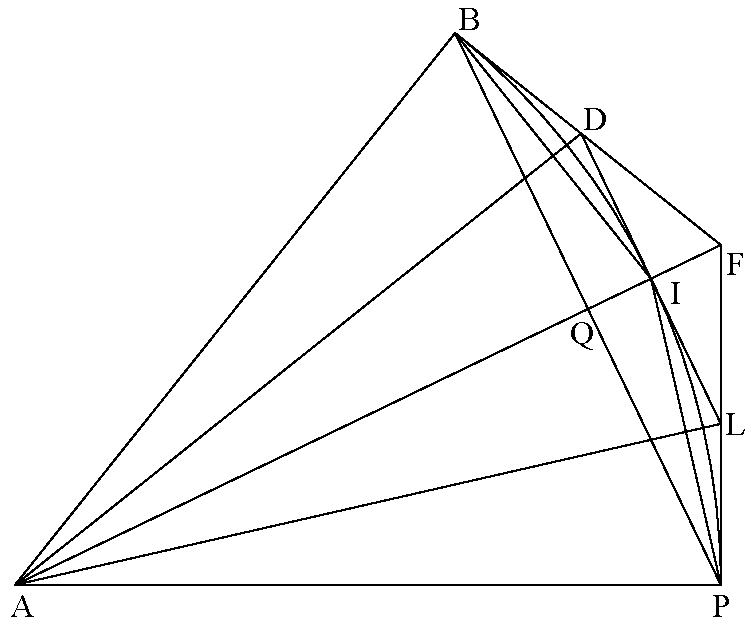
\includegraphics[scale=0.95]{vera_i}
\end{figure}

\newpage
\begin{samepage}
\begin{center}
\large\textsc{Proposition I. Theorem.}

\vskip 1.0em
\emph{The quadrilateral $BAPI$ is half of the quadrilateral $BAPF$ plus the
triangle $BAP$.}
\end{center}
\end{samepage}

The line $AQ$ is drawn through $F$ meeting with the the two lines $FB$ and $FP$,
which are tangent to the segment at the points $B$ and $P$. Therefore the line
$AQ$ contacts the line $BP$ at its bisector $Q$. We see from this that the triangle
$AQB$ is equal to the triangle $AQP$, the triangle $FBQ$ equals triangle
$FQP$, and the triangle $ABF$ equals triangle $APF$. Therefore the triangle
$ABF$ is half of the quadrilateral $ABFP$. Similarly the triangle $ABI$ is half
of the quadrilateral $ABIP$ and the triangle $ABQ$ is half of triangle $ABP$.
$ABF$, $ABI$, and $ABQ$ each have the same altitude and share one base, but the
other bases $AF$, $AI$, and $AQ$ progress arithmetically. Therefore the two
quadrilaterals $ABFP$ and $ABIP$ and the triangle $ABP$ are clearly in
arithmetic progression with a ratio of $AF$ to $AI$.

\vskip 1.0em
Let the line $DL$ be drawn tangent to the segment at the point $I$ so that it
will meet the lines $BF$ and $PF$ at the points $D$ and $L$, completing the
polygon $ABDLP$.

\begin{samepage}
\begin{center}
\large\textsc{Proposition II. Theorem.}

\vskip 1.0em
\emph{The quadrilateral $ABFP$ plus quadrilateral $ABIP$ is to the double of
quadrilateral $ABIP$ as quadrilateral $ABFP$ is to polygon $ABDLP$.}
\end{center}
\end{samepage}

The line $AF$ is drawn through the point of tangency of the line $DL$ with the
segment, and is likewise drawn through the meeting point of the two lines $FB$
and $FP$, which terminate the line $DL$ and touch the segment in two points.
Therefore the line $DL$ is bisected at the point $I$. Because of this the
triangle $FDI$ equals the triangle $FIL$ and the triangle $ABF$ equals the
triangle $APF$. Thus the quadrilateral $ABDI$ equals quadrilateral $APLI$, and
further quadrilateral $APLI$ is half of the polygon $ABDLP$. It is obvious from
the above demonstration that the triangle $AIL$ equals triangle $ALP$, but
triangle $ALF$ is to triangle $ALI$ as $FA$ is to $AI$ and $FA$ is to $AI$ as
quadrilateral $ABPF$ is to quadrilateral $ABIP$. Thus quadrilateral $ABFP$ is to
quadrilateral $ABIP$ as triangle $ALF$ is to triangle $AIL$. So putting it
together, quadrilateral $ABFP$ plus $ABIP$ is to quadrilateral $ABIP$ as
triangle $AFL$ plus triangle $AIL$, i.e. triangle $AFP$, is to triangle $AIL$.
Doubling this result, $ABFP$ plus $ABIP$ is to the double of $ABIP$ as triangle
$AFP$ is to quadrilateral $AILP$. Note that triangle $AFP$ is half of
quadrilateral $ABFP$ and quadrilateral $AILP$ is half of polygon $ABDLP$.
Therefore quadrilateral $ABFP$ plus quadrilateral $ABIP$ is to the double of
$ABIP$ as quadrilateral $ABFP$ is to polygon $ABDLP$.

\begin{samepage}
\begin{center}
\large\textsc{Proposition III. Theorem.}

\vskip 1.0em
\emph{The triangle $BAP$ plus the quadrilateral $ABIP$ is to the quadrilateral
$ABIP$ as the double of the quadrilateral $ABIP$ is to the polygon $ABDLP$.}
\end{center}
\end{samepage}

In the preceding proposition it is shown that the sum of $ABFP$ and $ABIP$ is to
the double of quadrilateral $ABIP$ as quadrilateral $ABFP$ is to polygon
$ABDLP$. By permuting we see that quadrilateral $ABFP$ plus $ABIP$ is to
quadrilateral $ABFP$ as the double of quadrilateral $ABIP$ is to polygon
$ABDLP$. Since quadrilaterals $ABFP$ and $ABIP$ and triangle $ABP$ are in
arithmetic progression, we have that quadrilateral $ABIP$ is to quadrilateral
$ABFP$ as triangle $ABP$ is to quadrilateral $ABIP$. Putting these together,
quadrilateral $ABIP$ plus $ABFP$ is to quadrilateral $ABFP$ as triangle $ABP$
plus quadrilateral $ABIP$ is to quadrilateral $ABIP$. On the other hand $ABIP$
plus $ABFP$ is to quadrilateral $ABFP$ as the double of quadrilateral $ABIP$ is
to polygon $ABDLP$. And therefore triangle $ABP$ plus quadrilateral $ABIP$ is
to quadrilateral $ABIP$ as the double of quadrilateral $ABIP$ is to polygon
$ABDLP$.

\vskip 1.0em
Let the lines $AD$ and $AL$ be drawn to meet the segment at the points $E$
and $O$ and intersecting the lines $BI$ and $IP$ at $H$ and $M$. From this are
joined the lines $BE$, $EI$, $IO$, and $OP$ to complete the polygon $ABEIOP$.

\begin{samepage}
\begin{center}
\large\textsc{Proposition IV. Theorem.}

\vskip 1.0em
\emph{The polygon $ABEIOP$ is half of $ABDLP$ plus the quadrilateral $ABIP$.}
\end{center}
\end{samepage}

From the previous theorem it is obvious that the quadrilateral $AILP$,
quadrilateral $AIOP$, and triangle $AIP$ are in arithmetic progression, and from
the previous proposition one can gather easily enough that the quadrilateral
$AILP$ is half of polygon $ABDLP$, quadrilateral $AIOP$ is half of polygon
$ABEIOP$, and triangle $AIP$ is half of quadrilateral $ABIP$. Thus by doubling
the terms, polygon $ABDLP$, polygon $ABEIOP$, and quadrilateral $ABIP$ are in
arithmetic progression.

\vskip 1.0em
Let lines $CG$ and $KN$ be drawn tangent to the segment at the points $E$ and
$O$ and let the lines $DL$, $DB$, and $LP$ intersect at the points $C$, $G$,
$K$, and $N$ to complete the polygon $ABCGKNP$.

\begin{samepage}
\begin{center}
\large\textsc{Proposition V. Theorem.}

\vskip 1.0em
\emph{The quadrilateral $ABIP$ plus the polygon $ABEIOP$ are to the polygon
$ABEIOP$ as the double of the polygon $ABEIOP$ is to the polygon $ABCGKNP$.}
\end{center}
\end{samepage}

From the third theorem it is obvious that the triangle $ABI$ plus the
quadrilateral $ABEI$ is to the quadrilateral $ABEI$ as the double of
quadrilateral $ABEI$ is to polygon $ABCGI$. From the previous proposition it is
easily concluded that triangle $ABI$ is half of quadrilateral $ABIP$,
quadrilateral $ABEI$ is half of polygon $ABEIOP$, and polygon $ABCGI$ is half of
polygon $ABCGKNP$. Therefore by doubling the terms, quadrilateral $ABIP$ plus
$ABEIOP$ is to polygon $ABEIOP$ as the double of polygon $ABEIOP$ is to polygon
$ABCGKNP$.

\vskip 1.0em
From this one can easily see that the polygon $ABCGKNP$ is the harmonic mean
between polygons $ABEIOP$ and $ABDLP$, which is sufficient to suggest that this
may be demonstrated in perpetuity.

\begin{samepage}
\begin{center}
\large\textsc{Scholium.}
\end{center}
\end{samepage}

The two preceding propositions can be proved by the same method for any such
complex polygons in place of the complex polygons $ABIP$ and $ABDLP$. Indeed the
tangent polygon contains as many equal quadrilaterals as the subtending polygon
contains triangles. And so it is evident that these ratios of the polygons
continue themselves to infinity, drawing lines $AN$, $AK$, $AG$, and $AC$
through points $R$, $T$, $S$, and $V$ and composing other lines and polygons
inside and outside of these. Note that we may say of these inscribed and
circumscribed polygons that they double by inscription and circumscription.

From the previous propositions it is obvious (if we let triangle $ABP = a$ and
quadrilateral $ABFP = b$) that quadrilateral $ABIP = \sqrt{ab}$ and polygon
$ABDLP = \frac{2ab}{a+\sqrt{ab}}$. By the same method, let quadrilateral $ABIP =
c$ and polygon $ABDLP = d$ and we have that polygon $ABEIOP = \sqrt{cd}$ and
polygon $ABCGKNP = \frac{2cd}{c+\sqrt{cd}}$. It is evindent from this
observation that the series of polygons converges.

And so, continuing this to infinity gives a magnitude equal to that of
the sector of the circle, the ellipse, or the hyperbola given by $ABEIOP$.
Indeed the difference of the complex polygons in the series always diminishes,
so that all of the magnitudes may be made smaller, as we shall demonstrate in
the theorems following the Scholium.

Therefore if the aforementioned series of polygons terminates, that is,
if one may find a final inscribed polygon (if we may call it that) equal to the
final circumscribed polygon, one would infallibly have the quadrature of the
circle and the hyperbola. But since it has proved difficult, and in geometry it
is perhaps altogether impossible for such a series to terminate, certain
propositions are given from which to find this kind of limit of the series.
After these (if it is possible) the general method for finding all of the
limits of convergent series will be given.

\begin{samepage}
\begin{center}
\large\textsc{Proposition VI. Theorem.}

\vskip 1.0em
\emph{The difference between the triangle $ABP$ and the quadrilateral $ABFP$
is greater than twice the difference between the quadrilateral $ABIP$ and the
polygon $ABDLP$.}
\end{center}
\end{samepage}

Denote the triangle $ABP$ by $A$, quadrilateral $ABFP$ by $B$, quadrilateral $ABIP$ by
$C$, and polygon $ABDLP$ by $D$. Since $A$ is to $C$ as $C$ is to $B$, the
difference between $A$ and $C$ is to $A$ as the difference between $C$ and $B$
is to $C$. Permuting, the difference between $A$ and $C$ is to the difference
between $C$ and $B$ as $A$ is to $C$. Now putting these together, the difference
between $A$ and $C$ plus the difference between $C$ and $B$, that is, the
difference between $A$ and $B$ is to the difference between $C$ and $B$ as $A+C$
is to $C$. But it has been shown that $A+C$ is to $C$ as $2C$ is to $D$ and the
difference between $A$ and $B$ is to the difference between $C$ and $B$ as $2C$
is to $D$. Since $A+C$ is to $C$ as $2C$ is to $D$, permuting gives $A+C$ is to
$2C$ as $C$ is to $D$.
Dividing, the difference between $A$ and $C$ is to $2C$ as the difference
between $C$ and $D$ is to $D$. Again permuting, the difference between $A$ and
$C$ is to the difference between $C$ and $D$ as $2C$ is to $D$. But now the
difference between $A$ and $B$ has been shown to be to the difference
between $C$ and $B$ as $2C$ is to $D$. So from this the difference between $A$
and $B$ is to the difference between $C$ and $B$ as the difference between $A$
and $C$ is to the difference between $C$ and $D$. However the difference between
$A$ and $B$ is greater than the difference between $C$ and $B$ so that the
difference between $A$ and $C$ is greater than the difference between $C$ and
$D$. Permuting the previous ratio, the difference between $A$ and $B$ is to the
difference between $A$ and $C$ as the difference between $C$ and $B$ is to the
difference between $C$ and $D$. The difference between $A$ and $B$ is greater
than the difference between $A$ and $C$ and so the difference between $C$ and
$B$ is greater than the difference between $C$ and $D$. But the difference
between $A$ and $B$ is equal to the difference between $A$ and $C$ plus the
difference between $C$ and $B$. Therefore either of them is greater than the
difference between $C$ and $D$ and so it is obvious that the difference between
$A$ and $B$ is greater than the double of the difference between $C$ and $D$,
that is, the difference between the triangle $ABP$ and the quadrilateral $ABFP$
is greater than twice the difference between the quadrilateral $ABIP$ and the
polygon $ABDLP$.

\begin{samepage}
\begin{center}
\large\textsc{Scholium.}
\end{center}

The same method may be used to demonstrate that the difference
between quadrilateral $ABIP$ and polygon $ABDLP$ is greater than twice the
difference between polygons $ABEIOP$ and $ABCGKNP$. By the same method
one can show that this difference is always exceeded in our halving
of the complex polygon to infinity. In fact the difference between the prior
inscribed and circumscribed polygons is always greater than twice the difference
between the subsequent inscribed and circumscribed polygons. Thus more than half
of the difference of the prior polygons is carried over to that of the
difference of the subsequent ones. Therefore continuing the halving of the
polygon, two complex polygons are found such that their difference is made
less than any given magnitude, as we obtained in the preceding Scholium.
\end{samepage}

Let there be two unknown magnitudes, $a$ and $b$, with $a$ less than $b$, and
let there be two given inequalities with $c$ greater than $d$ and $c$ 
greater than $e$. From here we have that $c$ is to $d$ as $b - a$ is to
$\frac{bd - ad}{c}$.  Then when $a$ is then added to the latter we get
$\frac{ca + bd - ad}{c}$, where the magnitude is immediately denoted $a$.
And also $c$ is to $e$ as $b - a$ is to $\frac{be - ae}{c}$. Then when this last
magnitude is subtracted from $b$ it yields $\frac{bc - be + ae}{c}$, which is
then denoted $b$.

One may continue the convergent series from here in which the first terms are
$a, b$ and the second are $\frac{ca+bd-ad}{c}, \frac{bc-be+ae}{c}$. It is
obvious that the term $\frac{ca+bd-ad}{c}$ is greater than the term $a$ since
the term $a$ is added to $\frac{bd-ad}{c}$ giving $\frac{ca+bd-ad}{c}$. It is
also clear that the term $\frac{ca+bd-ad}{c}$ is less than the term $b$ since the
difference between $a$ and $b$ is greater than the difference between $a$ and
$\frac{ca+bd-ad}{c}$. It is evident that the term $\frac{bc-be+ae}{c}$ is less
that the term $b$ since $\frac{be-ae}{c}$ is subtracted from $b$ giving
$\frac{bc-be+ae}{c}$. And it is further obvious that the term
$\frac{bc-be+ae}{c}$ is greater than $a$ since the difference between $a$ and
$b$ is greater than the difference between $\frac{bc-be+ae}{c}$ and $b$.
Therefore it is evident that the difference between the convergent terms $a$ and
$b$ is greater than the difference between the convergent terms
$\frac{ca+bd-ad}{c}$ and $\frac{bc-be+ae}{c}$.

However since the convergent terms $a$ and $b$ were given as unknown, $a$
and $b$ can be used in place of any of the convergent
terms of the whole of the series. So by putting $a$ and $b$ for any of the
terms, it necessarily follows from the composition of the
series that $\frac{ca+bd-ad}{c}$ and $\frac{bc-be+ae}{c}$ are the subsequent
convergent terms. And again since the difference between the terms $a$
and $b$ is greater than the difference between the terms $\frac{ca+bd-ad}{c}$
and $\frac{bc-be+ae}{c}$, it is clear that the difference between the
prior convergent term is always greater than the difference between the
subsequent convergent term. Because this difference always diminishes
proportionally in the ratio $b - a$ to $\frac{bc - be + ae - ca - bd +
ad}{c}$, one can see that the terms of this convergent series are always
decreasing. Therefore imagining this series continuing to infinity, we are able
to imagine the final convergent terms being equal, where we call these equal terms
the limit of the series.

\begin{samepage}
\begin{center}
\large\textsc{Proposition VII. Problem.}

\vskip 1.0em
\emph{To find the limit of the aforementioned series.}
\end{center}
\end{samepage}

In order to satisfy these problems, we first want to find a
magnitude that is composed by the same method from the convergent terms $a$ and
$b$ as from the convergent terms $\frac{ca+bd-ad}{c}$ and
$\frac{bc-be+ae}{c}$\footnote{That is, an invariant expression.}, which follows
easily from the following method.
The magnitude is found by a multiplication with $a$ and addition of $b$
times a magnitude $m$, and the same may be obtained by multiplication with
$\frac{ca+bd-ad}{c}$ and addition of $\frac{bc-be+ae}{c}$ times a magnitude $m$.
Let the magnitude be $z$, then $za+bm$ is equal to $\frac{zca + zbd - zad + mbc
- mbe + mae}{c}$ and the equation reduces to $z = \frac{mae - mbe}{ad - bd}$.
This magnitude whether multiplied by $a$ and added to $mb$, or multiplied by
$\frac{ca+bd-ad}{c}$ and added to $\frac{mbc-mbe+mae}{c}$ produces the same
magnitude in either case, namely $\frac{maae - mbae + mbad - mbbd}{ad -
bd}$\footnote{Here there is a typo in both editions of the book, giving the
denominator as $cd-bd$.}.
Thus the aforementioned magnitude is composed by the same method from the
convergent terms $a$ and $b$ as from the convergent terms $\frac{ca+bd-ad}{c}$
and $\frac{bc-be+ae}{c}$. Because $a$ and $b$ are unknown magnitudes they
can be any of the convergent terms of the series, where the subsequent
convergent terms are $\frac{ca+bd-ad}{c}$ and $\frac{bc-be+ae}{c}$.
Thus the magnitude $\frac{maae - mbae + mbad - mbbd}{ad - bd}$ is 
composed by the same method from any of the
convergent terms of the series given as $a$ and $b$. 
Therefore the this magnitude is composed in precisely the same way from its
final convergent terms, which are equal. 
Let this final term be $x$, which multiplied by $\frac{mae - mbe}{ad - bd}$ 
and by $m$ produces $xm$ and
$\frac{xmae - xmbe}{ad - bd}$. 
Summing the factors yields that $\frac{xmae - xmbe + xmad - xmbd}{ad - bd} 
= \frac{maae - mbae + mbad - mbbd}{ad - bd}$, and the equation
reduces to $x = \frac{aae - bae + bad - bbd}{ae - be + ad
- bd}$, which we wanted to find.

In order to make this problem less obscure we will illustrate with a numerical
exercise:
Let $c = 7$, $d = 2$, $e = 3$, $a = 28$, and $b = 42$. Then the second
convergent terms are $32$ and $36$, the third are $33\frac{1}{7}$ and
$34\frac{2}{7}$, and the limit is $33\frac{3}{5}$.

Changing nothing, if $a$ is less than $b$ then $\frac{ca+bd-ad}{c}$ may be
greater than $\frac{bc-be+ae}{c}$, indeed in analysis greater can be subtracted
by lesser, which is shown by this example: Let $c = 7$, $d
= 5$, $e = 4$, $a = 28$, and $b = 42$. The second convergent terms will be $38$
and $34$, the third $35\frac{1}{7}$ and $36\frac{2}{7}$, and the limit
$35\frac{7}{9}$.

Notice that the solution to this problem may even be obtained by the same
method if $a$ is zero. For example, let $c = 8$, $d = 3$, $e
= 4$, $a = 0$, and $b = 24$. Then the second convergent terms will be $9$ and
$12$, the third $10\frac{1}{8}$ and $10\frac{1}{2}$, and the limit of the series
$10\frac{2}{7}$.

Indeed the limits of these series can be found in Gregorie of St. Vincent's book
on geometric progression, although his way of proceeding differs greatly from
the one presented here.

\newpage
\begin{samepage}
\begin{center}
\large\textsc{Proposition VIII. Problem.}

\vskip 1.0em
\emph{Let the two quantities $A$ and $B$ be given and the ratio of $C$ to $D$ be
given. We want to find another magnitude so that the ratio of it to $A$ is the
multiplicate of the ratio of $B$ to $A$ in the ratio of $C$ to $D$.}\footnote{If
a ratio $x$ is the ``multiplicate'' of the ratio $y$ in the ratio $z$, then in modern notation $x = y^{z}$. Likewise, if a number $x$ is the ``submultiplicate'' of the ratio $y$ in
the ratio $z$, then in modern notation $x = y^{\frac{1}{z}}$. See
\cite[p.286]{Hutton}.}
\end{center}
\end{samepage}

First, let the ratio of $C$ to $D$ be commensurable, and let $E$ be a common
measure of $C$ and $D$. For as often as $E$ is contained in $D$ let the ratio of
$F$ to $A$ be the submultiplicate of the ratio of $B$ to $A$ in such
ratio
%\footnote{That is, $\frac{F}{A} = \left(\frac{B}{A}\right)^{\frac{D}{E}}$}
. Also as often as $E$ is contained in
$C$ let the ratio of $G$ to $A$ be the multiplicate of the ratio $F$ to $A$ in
such ratios
%\footnote{That is, $\frac{G}{A} = \left(\frac{B}{A}\right)^{\frac{C}{E}}$}
.
I claim that $G$ is the desired magnitude. The ratio of $G$ to $A$ is the
multiplicate of the ratio of $F$ to $A$ in the ratio of $C$ to $E$, and the
ratio of $F$ to $A$ is the multiplicate of the ratio of $B$ to $A$ in the ratio
of $E$ to $D$.
Therefore by equality, the ratio of $G$ to $A$ is the multiplicate of the ratio
$B$ to $A$ in the ratio $C$ to $D$, which is what we wanted to show.

If the ratio of $C$ to $D$ is incommensurable, then I am convinced that in
practice this problem is geometrically impossible. However it can be
accomplished by approximation, assuming a commensurable ratio that approaches
it.

Let there be a convergent series such that the first terms are $A$ and $B$, the
second $C$ and $D$, and the third $E$ and $F$. Let the second terms be made
by the first, where $B$ is greater than $A$, and the ratio of $B$ to $A$ is the
multiplicate of the ratio of $C$ to $A$ in the ratio of $M$ to $N$, with $M$
greater than $N$, and likewise the ratio of $B$ to $A$ is the multiplicate of
the ratio of $D$ to $A$ in the ratio of $M$ to $O$, with $M$ greater than $O$.
Let it follow that the third terms are made from the second as the second are
made from the first, and so the series continues.

\begin{samepage}
\begin{center}
\large\textsc{Proposition IX. Problem.}

\vskip 1.0em
\emph{To find the limit of the aforementioned series.}
\end{center}
\end{samepage}

Let $G$ be zero, that is the exponent of the ratio of equality, or of the ratio
of $A$ to $A$.
Also let $H$ satisfy the exponent of the ratio of $B$ to $A$. 
Let the ratio of $M$ to $N$ be the ratio of the difference between $G$ and $H$,
which is $H$ itself, or the exponent of the ratio $B:A$, to the difference
between $G$ and $I$, which is $I$ itself. 
But the ratio of $M$ to $N$ is the ratio by which the ratio of $B$ to $A$ is the
multiplicate of the ratio of $C$ to $A$.
Therefore the excess of $I$ over $G$, which is $I$ itself, is the exponent of
the ratio of $C$ to $A$. 
Let the ratio of $M$ to $O$ be as the ratio of the excess of $H$ over $G$, which
is $H$, to the excess of $K$ over $G$, which is $K$. 
But then the ratio of $M$ to $O$ is the ratio by which the ratio of $B$ to $A$
is the multiplicate of the ratio of $D$ to $A$. 
Whenever $H$ is the exponent of the ratio of $B$ to $A$, $K$ will be the
exponent of the ratio of $D$ to $A$.
Therefore if $I$ is the exponent of the ratio of $C$ to $A$ and $K$ is the
exponent of the ratio of $D$ to $A$, then the excess of $K$ over $I$ will be the
exponent of the ratio of $D$ to $C$. 
From here let the ratio of $M$ to $N$ be as the excess of $K$
over $I$, or the exponent of the ratio of $D$ to $C$, is to the excess of $R$
over $I$. 
Then the ratio of $M$ to $N$ is the ratio, from the composition of the series,
by which the ratio of $D$ to $C$ is the multiplicate of the ratio of $E$ to $C$,
and so the excess of $K$ over $I$ is the exponent of the ratio of $D$ to $C$.
Thus the excess of $R$ over $I$ is the exponent of the ratio of $E$ to $C$ and
$I$ is the exponent of the ratio of $C$ to $A$.
Therefore $R$ is the exponent of the ratio of $E$ of $A$. 
From here let the ratio of $M$ to $O$ be
as the excess of $K$ over $I$ is to the excess of $S$ over $I$.
Then the ratio of $M$ to $O$ is the ratio, from the composition of the series,
by which the ratio of $D$ to $C$ is the multiplicate of the ratio of $F$ to $C$,
where the excess of $K$ over $I$ is the exponent of the ratio of $D$ to $C$. 
The excess of $S$ over $I$ will be the exponent of the ratio of $F$ to $C$ and
$I$ is the exponent of the ratio of $C$ to $A$. Thus $S$ is the exponent of the
ratio of $F$ to $A$. 
Therefore when $R$ is the exponent of the ratio of $E$ to $A$ and $S$ is the
exponent of the ratio of $F$ to $A$, the excess of $S$ over $R$ will be the
exponent of the ratio of $F$ to $E$. Continuing the series, it may be shown as
before that $T$ is the exponent of the ratio of $X$ to $A$ and $V$ the exponent
of the ratio of $Y$ to $A$. Finally it will always be the case that the
convergent terms of the series of exponents are exponents of the ratios of any
convergent terms of the series may be found in the same way by the initial
values, and specifically of the convergent terms of the proposed series by the
first magnitude $A$ of the series.
Thus by the limit of the series of exponents is found by 7. 
For example, let $L$ be the limit of the proposed series with the first term
$A$, then it will be the exponent of the ratio. 
Therefore the ratio of $Z$ to $A$ may be found, and is the multiplicate of
the given ratio of $B$ to $A$ in the ratio of $L$ to $H$, and $Z$ will be the
desired limit, which we wanted to find.

To illustrate this problem in numbers, let $M = 4$, $N = 2$, $O = 1$, $A = 6$,
and $B = 10$. Then the second convergent terms shall be $\sqrt{60}$ and
$\left(2160\right)^{\frac{1}{4}}$, the third convergent terms
$\left(7776000\right)^{\frac{1}{8}}$ and
$\left(100776960000000\right)^{\frac{1}{16}}$, and the limit of the series
$\left(360\right)^{\frac{1}{3}}$.

As another example, let $M = 6$, $N = 2$, $O = 3$, $A = 5$, and $B = 10$. Then
the second convergent terms of the series shall be
$\left(250\right)^{\frac{1}{3}}$ and $\sqrt{50}$, the third
$\left(488281250000000\right)^{\frac{1}{18}}$ and
$\left(7812500000\right)^{\frac{1}{12}}$, and the limit of the series
$\left(12500\right)^{\frac{1}{5}}$. So far all of the limits of the convergent
series can be made either by a single arithmetic proportion or a single
geometric proportion. Now I shall add to the method, and by the power of this
addition the limits of all convergent series may be found.

\newpage
\begin{samepage}
\begin{center}
\large\textsc{Proposition X. Problem.}

\vskip 1.0em
\emph{To find the limit of a given convergent series from a given magnitude
composed by the same method from two convergent terms of the series as from the
subsequent convergent terms of the same series.}
\end{center}
\end{samepage}

Let the convergent series be of any two convergent terms $a$ and $b$ and the
subsequent convergent terms $\sqrt{ab}$ and $\frac{aa}{\sqrt{ab}}$. The sum
of the convergent terms $a+b$ multiplied by the first convergent term $a$ gives
$aa+ab$. The sum of the subsequent convergent terms
$\sqrt{ab}+\frac{a^{2}}{\sqrt{ab}}$ multiplied by the first convergent term
$\sqrt{ab}$ likewise gives $aa+ab$. From this is discovered the limit of
the convergent series. It is clear that the magnitude $aa+ab$ is made by
the same method from the convergent terms $a$ and $b$ as from the subsequent
convergent terms $\sqrt{ab}$ and $\frac{aa}{\sqrt{ab}}$, and because the
magnitudes $a$ and $b$ were arbitrary terms of the convergent series,
it is evident that the sum of any proposed convergent terms of the series
multiplied by the first convergent term will give that same magnitude, which is
likewise the sum of the subsequent convergent terms multiplied by the first
convergent term. Since two convergent terms are always followed by two
convergent terms, it is clear that the sum of any two of the convergent
terms multiplied by the first convergent term will be $aa+ab$. And so the
final convergent terms are equal. Therefore let the final term of this series be
the limit $z$, which is added to itself and the sum multiplied by itself to give
$2zz$, which equals the magnitude $aa+ab$, and solving this equation
for $z$ yields the limit of the series $\sqrt{\frac{aa+ab}{2}}$, which we
wanted to find.

And therefore in order to find the limit of any convergent series it is
necessary only to discover a magnitude composed by the same method from the
first convergent terms as from the second convergent terms.

\begin{samepage}
\begin{center}
\large\textsc{Corollary.}
\end{center}

Since it is not important to the problem whether the convergent terms $a$ and
$b$ are the first, second, third, etc., it is clear that all of the convergent
terms of the series are composed by the same method from the first convergent
terms as by the second, third, fourth, etc. convergent terms.
\end{samepage}

\begin{samepage}
\begin{center}
\large\textsc{Proposition XI. Theorem.}

\vskip 1.0em
\emph{The sector of the circle, ellipse, or hyperbola $ABIP$ is not composed
analytically by the triangle $ABP$ and the quadrilateral $ABFP$.}
\end{center}
\end{samepage}

Let the triangle $ABP = a$ and the quadrilateral $ABFP = b$. 
It is clear from the preceding propositions that the quadrilateral $ABIP =
\sqrt{ab}$ and the polygon $ABDLP = \frac{2ab}{a+\sqrt{ab}}$. 
The sector $ABIP$ is the limit of this convergent series. 
So that the radical signs and fractions may be removed from the
terms of the series, for the first convergent terms of the series $a$ and $b$,
that is, for the triangle $ABP$ and the quadrilateral $ABFP$, put $a^{3}+a^{2}b$
and $a^{2}b+b^{3}$. 
Then the second convergent terms of the series, which are the
quadrilateral $ABIP$ and the polygon $ABDLP$, will be $ba^{2}+b^{2}a$ and 
$2b^{2}a$. 
I claim that the limit of the convergent series (where the first convergent
terms of the series are $a^{3}+a^{2}b$ and $a^{2}b+b^{3}$ and the second are
$ba^{2}+b^{2}a$ and $2b^{2}a$) is not composed analytically of the terms
$a^{3}+a^{2}b$ and $a^{2}b+b^{3}$\footnote{Here Gregory mens that he cannot,
as in the previous example, devise an invariant expression in which he can
solve for the limit, which is to say he cannot devise an analytic expression
for the limit where he would obtain the same expression whether substituting
the first pair of terms or the second pair of terms of the series.}.
Indeed, if the aforementioned limit is composed analytically of the terms
$a^{3}+a^{2}b$ and $a^{2}b+b^{3}$, then the limit would itself be analytic and
would be composed in the same way from the convergent terms $ba^{2}+b^{2}a$
and $2b^{2}a$. 
Therefore the limit would be composed analytically in the same way
from $a^{3}+a^{2}b$ and $a^{2}b+b^{3}$ as it is composed from $ba^{2}+b^{2}a$
and $2b^{2}a$, but no magnitude may be composed analytically in the same way
from $a^{3}+a^{2}b$ and $a^{2}b+b^{3}$ as it is composed from $ba^{2}+b^{2}a$
and $2b^{2}a$, which I now demonstrate. 
If a magnitude may be composed analytically in the same
way from $a^{3}+a^{2}b$ and $a^{2}b+b^{3}$ as it is composed from
$ba^{2}+b^{2}a$ and $2b^{2}a$, then it would be produced by the adding,
subtracting, multiplying, dividing, and the extraction of square roots from the
terms $a^{3}+a^{2}b$ and $a^{2}b+b^{3}$ as if in the same way the terms
$ba^{2}+b^{2}a$ and $2b^{2}a$ were added, subtracted, multiplied, divided, and
the square roots extracted. 
However the latter is not possible to do, so neither can be the former. 
Thus I prove the latter: if the same magnitude would be made by
addition, subtraction, multiplication, division, and the extraction of square
roots of the terms $a^{3}+a^{2}b$ and $a^{2}b+b^{3}$, which themselves are made
by addition, subtraction, multiplication, division, and the extraction of square
roots of the terms $ba^{2}+b^{2}a$ and $2b^{2}a$, then by adding, or
subtracting, or multiplying, or dividing equal magnitudes by or to the terms
$a^{3}+a^{2}b$ and $a^{2}b+b^{3}$, or by the extraction of square roots, these
analytic operations being substituted in some way, by their reiteration or by
both of these or by doing none of them, the two terms can be made into the final
result, one from the term $a^{2}b+b^{3}$ and the other from the term $2b^{2}a$. 
Thus the final result from the term $a^{3}+a^{2}b$ with the final result from
$a^{2}b+b^{3}$ is the same as the final result by the term $ba^{2}+b^{2}a$ with
the final result from the term $2b^{2}a$ in the same way added, subtracted,
multiplied, divided, and square roots extracted.
This, however, is absurd, and therefore so is the earlier claim.
That which follows is mostly made clear by the eighth definition, by which
prove the rest.
In the term $a^3+a^2b$ is found a power of $a$, namely $a^3$, which is higher
than any power of $a$ found in the term $ba^2+b^2a$, and therefore also when
equal magnitudes by addition, subtraction, multiplication, division, etc. to
the terms $a^3+a^2b$ and $ba^2+b^2a$.
Just as it has been declared above, it will always be that the powers of $a$ in
the final result from the term $a^3+a^2b$ will be higher than the powers of $a$
in the final product from the term $ba^2+b^2a$ because by adding, subtracting,
multiplying, dividing, etc. to those with equal magnitudes always results in the
making the same powers, and in the same way multiplying to those always elevates
the higher powers in the term $a^3+a^2b$ higher still than the lower powers in
the term $ba^2+b^2a$, and also in extracting the same square roots from these,
when $a$ is higher in power, it will be higher also in the square root.
And so because the highest power of $a$ is found in the term
$ab^2+b^3$ **than which is found in the term $2b^2a$, it is shown as before the
highest power of $a$ in the final result from the term $ab^2+b^3$ is the same as
the highest power of $a$ in the final result from the term $2b^2a$.
Therefore in the final result of the term $a^3+a^2b$ is found higher powers of
$a$ than in the final result of the term $ba^2+b^2a$, and in the final result of
the term $ab^2+b^3$ the highest powers of $a$ is the same with the highest power
of $a$ in the final result of the term $2b^2a$.
And therefore the final result from the terms $a^3+a^2b$ and $ab^2+b^3$, added,
subtracted, multiplied, divided, etc. between them in the same way, will always
produce a magnitude in which is found higher powers of $a$ than any of those
which can be found in the given magnitude by straight forward
addition, subtraction, multiplication, division, etc. of the results from the
terms $ba^2+b^2a$ and $2b^2a$ because the higer powers taken with another power
always makes a higher power than the lower powers with the same other power.
And therefore these two magnitudes cannot be identically equal, when higher
powers of $a$ may be found the in one term than in the other.
And so it is clear that the sector of the circle, ellipse, or hyperbola
$ABIP$ cannot be composed analytically from the triangle $ABP$ and the
quadrilateral $ABFP$, as was to be shown.

However, so that the proposition may be made perfectly clear, I subject it to
a more brief and easier proof stemming from another means of attack. A
magnitude cannot be composed analytically from the terms $a^{3}+a^{2}b$ and
$a^{2}b+b^{3}$ in the same way as it is composed from the
terms $ba^{2}+b^{2}a$ and $2b^{2}a$ because by the adding, subtracting,
multiplying, and dividing of the two numbers $a^{3}+a^{2}b$ and $a^{2}b+b^{3}$,
and by extracting square roots, more terms are made in the end result than if
the binomial $ba^2+b^2a$ and the simple magnitude $2b^2a$ are added, subtracted,
multiplied, divided, or square roots extracted.  So if more terms are in one
result than the other, it is impossible that they are identically equal, which
was proposed. The rest of the claim can be obtained from the prior proof.

\begin{samepage}
\begin{center}
\large\textsc{Scholium.}
\end{center}

This theorem will perhaps be seen as most obscure because of the many unusual
expressions that need to be employed, and because of the many lemmas assumed,
which were indeed irksome to prove, since to any analyst they are obvious
upon a first reading, as they follow entirely from the nature of analytic
operations.

This position requires that I speak to some degree on the proportion between
the triangle $ABP$ and the quadrilateral $ABIP$, because as it so happens,
drawing attention to the truest axiom of the philosophers, all of
our inquiry originates in the perceiving.
Indeed between the kinds of proportions, the perceiving of the the commensurable
only needing to be touched upon in order to be understood completely by the
human mind, but the incommensurable thus far being only barely contemplated by
mathematicians, so far as a commensurable ratio of a certain thing is
subdublicated, subtriplicated, etc. or born from addition, subtraction, etc.
That is, a magnitude which is incommensurable to a given magnitude from it is
only barely contemplated by human minds, since the commensurable can be composed
from other of the known and given magnitudes by addition, subtraction,
multiplication, division, and square root extraction.
And from the proofs thus far it is clear that the sector $ABIP$ cannot be
composed from addition, subtraction, multiplication, division, and square root
extraction from the triangle $ABP$ and the quadrilateral $ABFP$.
However the triangle $ABP$ and the quadrilateral $ABFP$ we suppose to be
mutually analytic magnitudes, and thus the sector $ABIP$ cannot be analytic to
these, which is to say it cannot be composed analytically from the magnitudes
$ABP$ and $ABFP$ by addition, subtraction, multiplication, division, and the
extraction of square roots.
Therefore because of this, noone can exhibit the ratio between the
triangle $ABP$ and the sector $ABIP$, since it is clear that this ratio is not
analytic.
But it will be claimed strongly by some that the ratio between the triangle
$ABP$ and the sector $ABIP$ can be changed in any way, and thus the ratio
between them could be analytic or even commensurable depending on how they are
given.
I respond that if this were the case the ratio between the triangle $ABP$ and
the quadrilateral $ABFP$ will not be analytic.
Therefore the triangle $ABP$ will never be given in analytic terms from a given
circle, ellipse, or hyperbola, which is most clear from the preceding.
However, even if from the preceding we cannot fully comprehend the ratio between
the triangle $ABP$ and the sector $ABIP$, we can come to know it to a great
extent because the sector $ABIP$ is the limit of the given convergent series.
And from this consideration it is possible to find a commensurable magnitude
whose difference from the sector $ABIP$ will be less than any
given magnitude.
It always returns to this when the practicioners work with incommensurable
magnitudes, and in this our practice of approximation will not be more laborious
than in the many other approximations of analytic magnitudes, and indeed it will
be even easier, shorter, and better equipped than that of the angular section of
Viète, which the greatest mathematicians are beginning to use again in practice.
Thus I do not see how the quadrature of the circle is to be considered unknown
any longer.
Since indeed it has been shown that the ratio of the circle to the square of the
diameter is not analytic, it will certainly be vain and inept to try to find, as
it were, such an impostor.
And in face of the rejection of such an analytic magnitude, I hardly believe
that any can be better known than by this convergent series of ours, insofar as
it is most plainly given by such a sequence.
\end{samepage}

\begin{center}
\large\textsc{Proposition XII. Theorem.}
\end{center}

\begin{figure}[h]
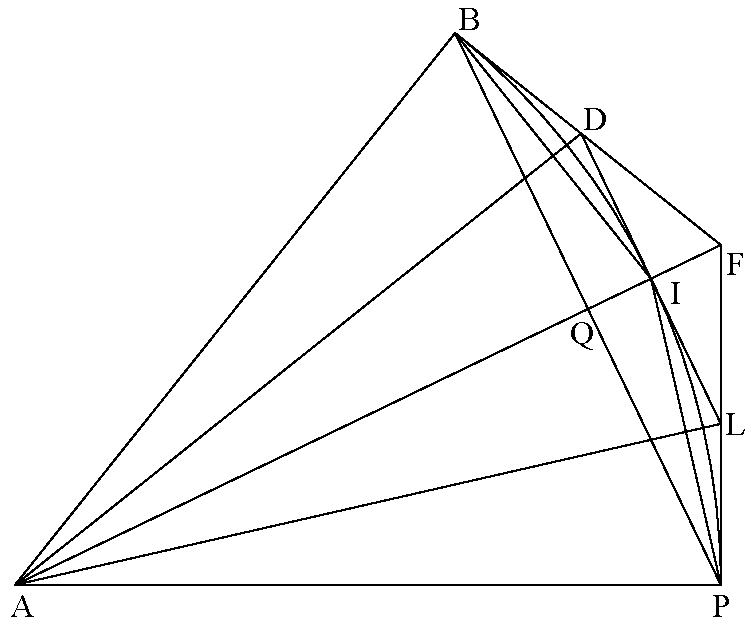
\includegraphics[scale=0.95]{vera_i}
\end{figure}

\vskip 1.0em
Let the quadrilateral $ABIP$ be $A$, the polygon $ABEIOP$ be $C$,
the polygon $ABCGKNP$ be $D$, and the polygon $ABDLP$ be $B$. 
I claim that $D$ is the harmonic mean of $C$ and $B$. 
Combining proposition 4 and $A:C::C:B$ gives $A+C:C::C+B:B$. 
But then from proposition 5, $A+C:C::2C:D$ and also $C+B:B::2C:D$. 
Permuting gives $B+C:2C::B:D$ and by dividing, the difference between $B$ and
$C$ is to $2C$ as the difference between $B$ and $D$ is to $D$. 
Again by permuting, the difference between $B$ and $C$ is to the difference
between $B$ and $D$ as $2C$ is to $D$, that is, as $C+B$ is to $B$. 
And by dividing, the difference between $D$ and $C$ is to the difference between
$B$ and $D$ as $C$ is to $B$. 
Therefore $D$ is the harmonic mean between $C$ and $B$, as was to be shown.

This proposition holds in the same way for each complex polygon, as the
Scholium of Proposition 5 explains.

\begin{center}
\large\textsc{Proposition XIII. Theorem.}
\end{center}

\vskip 1.0em
Let $C$ be the arithmetic mean, $D$ the geometric mean, and $E$ the harmonic
mean of the two magnitudes $A$ and $B$. 
I claim that $C$, $D$, and $E$ are continuously proportional
\footnote{That is, $C:D::D:E$.}. 
Because $A$, $E$, and $B$ are in harmonic ratio, the difference between $A$ and
$E$ shall be to the difference between $E$ and $B$ as $A$ is to $B$. 
Combining these, the difference between $A$ and $B$ shall be to the difference
between $E$ and $B$ as $A+B$ is to $B$. 
Now by permuting and combining, $2A:A+B::E:B$, but $2A$ is twice $A$ and
$A+B$ is twice $C$, so that $A:C::E:B$. 
Thus $CE=AB$ and $AB=DD$, and so $CE=DD$. 
Therefore $C:D::D:E$, as was to be shown.

\begin{figure}[h]
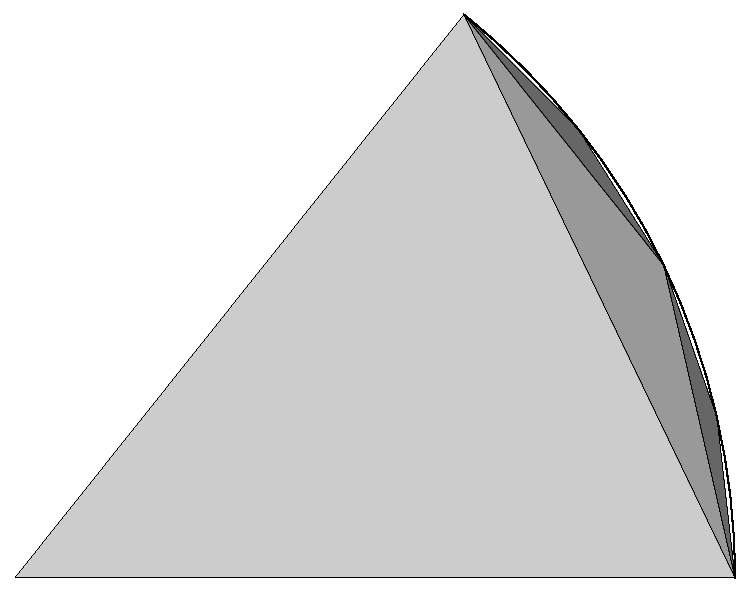
\includegraphics[scale=0.95]{vera_inscr}
\caption*{Series of inscribed polygons.}
\end{figure}

\begin{center}
\large\textsc{Proposition XIV. Theorem.}
\end{center}

\vskip 1.0em
Let $A$ and $B$ be two complex polygons with $A$ inscribed in the sector of a
circle or ellipse and $B$ circumscribed. 
A convergent series of these complex polygons may be continued according to our
method of drawing the subdouble, so that the polygons inscribed in the circle
are $A$, $C$, $E$, etc. and those circumscribed are $B$, $D$, $F$, etc. 
I claim that $A+E$ is less than $2C$.
This is clear from the previous propositions by the following analogies.
First, $A$, $C$, and $B$ are continuously proportional, and second $C$, $D$, and
$B$ are in harmonic proportion. 
Therefore the excess of $C$ over $A$, that is $C-A$, is to the excess of $D$
over $C$, or $D-C$, in a ratio composed from the proportion $A:C$ and from the
proportion $A+C:A$, that is in the ratio $A+C:C$. 
And $A+C$ is greater than $C$, so that the excess of $C$ over $A$ is greater
than the excess of $D$ over $C$.
However $D$ is greater than $E$ and so the excess of $C$ over $A$ is
much greater than the excess of $E$ over $C$. Therefore $A+E$ is less
than $2C$, as was to be shown.

\begin{figure}[h]
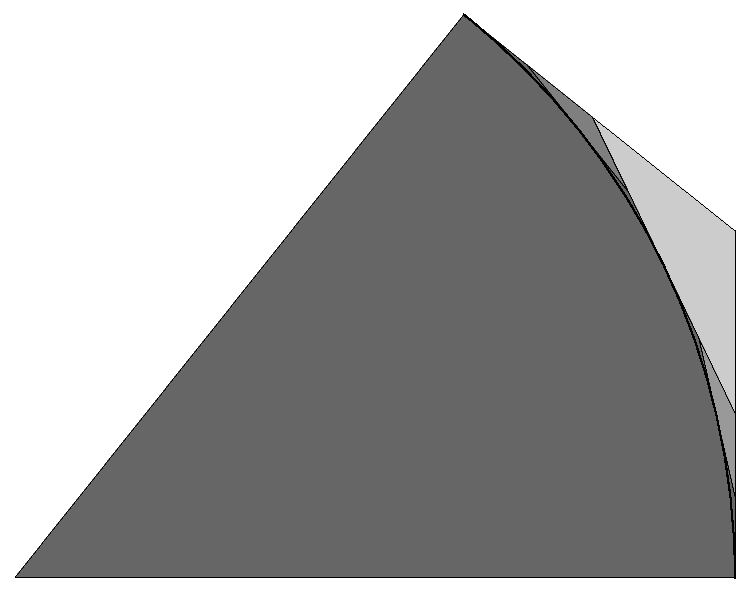
\includegraphics[scale=0.95]{vera_circumscr}
\caption*{Series of circumscribed polygons.}
\end{figure}

\begin{center}
\large\textsc{Proposition XV. Theorem.}
\end{center}

\vskip 1.0em
By the same assumptions, I claim that the excess of $C$ over $A$ is
less than the quadruple of the excess of $E$ over $C$. 
This is clear from the previous propositions by analogy with the following three
analogies. 
First, $A$, $C$, and $B$ are continuously proportional, second $C$, $D$, and
$B$ are in harmonic proportion, and third $C$, $E$, and $D$ are continuously
proportional. 
And so the excess of $C$ over $A$, that is $C-A$, is to
the excess of $E$ over $C$, or $E-C$, as $AC+EC+AE+CC$ is to $CC$,
and $B$ is greater than $E$. 
So $AB$, or $CC$, is greater than $AE$, and thus
$AE+CC$ is less than $2CC$. 
And so $AC+EC$ is to $2CC$ as $A+E$ is to $2C$, but
$A+E$ is less than $2C$ so that $AC+EC$ is less than $2CC$. 
Thus $AC+EC+AE+CC$ is less than $4CC$. 
Therefore $C-A$ is less than the quadruple of $E-C$, as was to be shown.

\begin{center}
\large\textsc{Proposition XVI. Theorem.}
\end{center}

\vskip 1.0em
Let $A$ and $B$ be two complex polygons with $A$ circumscribed about the sector
of a hyperbola and $B$ inscribed. 
A convergent series of these complex polygons
may be continued according to our method of drawing the subdouble, so that the
polygons circumscribed about the hyperbola are $A$, $C$, $E$, etc. and those
inscribed are $B$, $D$, $F$, etc. 
I claim that $A+E$ is greater than $2C$. 
This is clear from the previous propositions by the following analogies. 
First, $A$, $C$, and $B$ are continuously proportional, and 
second $C$, $D$, and $B$ are in harmonic proportion. 
Therefore the excess of $A$ over $C$, that is $A-C$, is to 
the excess of $C$ over $D$, or $C-D$, in a ratio composed from 
the proportion $A:C$ and from the proportion $A+C:A$, that is in the ratio
$A+C:C$. 
And $A+C$ is greater than $C$, so that the excess of $A$ over $C$ is greater
than the excess of $C$ over $D$. 
However $E$ is greater than $D$ and so the excess of $A$ over $C$ is much
greater than the excess of $C$ over $E$. Therefore $A+E$ is greater
than $2C$, as was to be shown.

\begin{center}
\large\textsc{Proposition XVII. Theorem.}
\end{center}

\vskip 1.0em
By the same assumptions, I claim that the excess of $A$ over $C$ is
greater than the quadruple of the excess of $C$ over $E$. 
This is clear from the previous propositions by analogy with the following three
analogies. 
First, $A$, $C$, and $B$ are continuously proportional, second $C$, $D$, and
$B$ are in harmonic proportion, and third $C$, $E$, and $D$ are continuously
proportional. 
And so the excess of $A$ over $C$, that is $A-C$, is to
the excess of $C$ over $E$, or $C-E$, in a ratio composed of the
proportions $A:C$, $A+C:A$, and $E+C:C$. 
And so $A-C$ is to $C-E$ as $AC+EC+AE+CC$ is to $CC$, and $B$ is less than $E$.
So $AB$, or $CC$, is less than $AE$, and thus $AE+CC$ is greater than $2CC$. 
And so $AC+EC$ is to $2CC$ as $A+E$ is to $2C$, but $A+E$ is greater than $2C$
so that $AC+EC$ is greater than $2CC$. 
Thus $AC+EC+AE+CC$ is greater than $4CC$. 
Therefore $C-A$ is greater than the quadruple of $E-C$, as was to be shown.

\begin{center}
\large\textsc{Proposition XVIII. Theorem.}
\end{center}

\vskip 1.0em
Let $A$ and $B$ be two magnitudes such that $A$ is less than $B$. 
Let $C$ be their geometric mean and $D$ their arithmetic mean. 
I claim that $D$ is greater than $C$. 
Since $B$, $C$, and $A$ are continuously proportional, by dividing, permuting,
and combining, it shall be that the excess of $B$ over $A$ is to the excess of
$C$ over $A$ as $A+C$ is to $A$. 
And so $A+C$ is greater than twice $A$. 
Thus the excess of $B$ over $A$ is greater than twice the excess 
of $D$ over $A$, so that the excess of $D$ over $A$ is greater than 
the excess of $C$ over $A$.
Therefore $D$ is greater than $C$, as was to be shown.

\begin{center}
\large\textsc{Proposition XIX. Theorem.}
\end{center}

\vskip 1.0em
By the same assumptions, let $E$ be the harmonic mean of $A$ and $B$. 
I claim that $C$ is greater than $E$. 
From proposition 13, $D$ is to $C$ as $C$ is to $E$, but $D$ is greater than
$C$. 
Therefore $C$ is greater than $E$, as was to be shown.

\begin{center}
\large\textsc{Corollary.}
\end{center}

\vskip 1.0em
From the two preceding propositions it is obvious that $D$ is greater than $E$,
that is, that the arithmetic mean of two magnitudes is greater than the harmonic
mean of the same.

\begin{center}
\large\textsc{Proposition XX. Theorem.}
\end{center}

\vskip 1.0em
Let $A$ and $B$ be two complex polygons with $A$ inscribed in the sector of a
circle or ellipse and $B$ circumscribed. 
A convergent series of these complex polygons may be continued according to our
method of drawing the subdouble, so that the polygons inscribed in the circle
are $A$, $C$, $E$, $K$, etc. and those circumscribed 
are $B$, $D$, $F$, $L$, etc. 
Also let $Z$ be the limit of the convergent series, that is, the sector of the
circle or ellipse. 
I claim that $Z$ is greater than $C$ plus one third of the 
excess of $C$ over $A$.
Let the excess of $G$ over $C$ be a fourth part of the excess of
$C$ over $A$ and the excess of $H$ over $G$ be a fourth part of
the excess of $G$ over $C$. 
This series may be continued to infinity, so let $X$ be the limit of this
process. 
The excess of $C$ over $A$ is less than the quadruple of the excess of $E$ over
$C$, and so the excess of $E$ over $C$ is greater than the excess
of $G$ over $C$, and therefore $E$ is greater than $G$. 
Now the excess of $E$ over $C$ is less than the quadruple of the excess of $K$
over $E$, and so the excess of $G$ over $C$ is much less than the excess of $K$
over $E$, and therefore the excess of $K$ over $E$ is greater than the excess of
$H$ over $G$.
Since $E$ is greater than $G$, it is obvious $K$ is greater than $H$. 
It is demonstrated in the same way for every series $A$, $C$, $E$ and $A$,
$C$, $G$, by continuation to however many terms. 
Each term of the series $A$, $C$, $E$ is greater than the corresponding term of
the series $A$, $C$, $G$. 
And so the limit of the series $A$, $C$, $E$, that is $Z$, will be greater than
the limit of the series $A$, $C$, $G$, that is $X$. 
And from Archimedes, the quadrature of the parabola corresponding to $X$ is
equal to $C$ plus one third of the excess of $C$ over $A$, and therefore $Z$ is
greater than this, as was to be shown.

\begin{center}
\large\textsc{Proposition XXI. Theorem.}
\end{center}

\vskip 1.0em
By the same assumptions as above, I claim that $Z$, which is a sector of a
circle or ellipse, is less than the greater of the two continuously
proportional arithmetic means of $A$ and $B$. 
Let $G$ be the arithmetic mean of $A$ and $B$ and $H$ be the arithmetic mean
between $G$ and $B$. 
Likewise let $M$ be the arithmetic mean of $G$ and $H$ and $N$ be the
arithmetic mean of $M$ and $H$. 
This convergent series, with terms $AB$, $GH$, $MN$,
$OP$, may be continued infinitely, so that its limit is $X$. 
It is clear from the preceding propositions that $G$ is greater than $C$, and
$H$, the arithmetic mean of $G$ and $B$, is greater than the harmonic mean of
$G$ and $B$. 
However the harmonic mean of $G$ and $B$ is greater than $D$, the harmonic
mean of $C$ and $B$, since $G$ is greater than $C$. 
And so the arithmetic mean of $G$ and $B$, that is $H$, is greater than $D$, the
harmonic mean of $C$ and $B$. 
By the same method $M$, the arithmetic mean of $G$ and $H$ is greater than
the geometric mean between $G$ and $H$. 
And since $G$ is greater than $C$, and $H$ is greater than $D$, the geometric
mean of $G$ and $H$ is greater than $E$, the geometric mean of $C$ and $D$. 
Thus $M$ is greater than $E$. 
Now $N$, the arithmetic mean of $M$ and $H$, is greater than the harmonic mean
of the same, and since $H$ is greater than $D$ and $M$ is greater than $E$, the
harmonic mean of $M$ and $H$ is greater than $F$, the harmonic mean of $E$ and
$D$. 
And so $N$ is greater than $F$. 
Continuing the series in the same way to infinity, one
may always show that the terms of the series $AB$, $CD$ are less
than the corresponding terms of the series $AB$, $GH$. 
Therefore the limit, $Z$, of the series $AB$, $CD$ will be less than the
limit, $X$, of the series $AB$, $GH$. 
Also, from Proposition 7, the limit, $X$, of the series $AB$, $GH$ is equal to
the greater of the two continuously proportional arithmetic means of $A$ and
$B$, and so $Z$ is the less than the same, as was to be shown.

\begin{center}
\large\textsc{Proposition XXII. Theorem.}
\end{center}

\vskip 1.0em
By the same assumptions as above, I claim that I claim that $Z$, which is a
sector of a circle or ellipse, is less than the greater of the two continuously
proportional geometric means of $A$ and $B$. 
Let $G$ be the geometric mean of $A$ and $B$ and $H$ be the geometric mean
between $G$ and $B$. 
Likewise let $M$ be the geometric mean of $G$ and $H$ and $N$ be the geometric
mean of $M$ and $H$. 
This convergent series, with terms $AB$, $GH$, $MN$,
$OP$, may be continued infinitely, so that its limit is $X$. 
It is clear from the preceding propositions that $C$ and $G$ are equals, and $H$
is greater than $D$. 
By this reasoning, $M$, the geometric mean of $G$ and $H$, is greater
than $E$, the geometric mean of $C$ and $D$. 
Now $N$, the geometric mean of $M$ and $H$, is greater than the harmonic mean of
the same, and since $M$ is greater than $E$ and $H$ is greater than $D$, the
harmonic mean of $M$ and $H$ is greater than $F$, the harmonic mean of $E$ and
$D$. 
And so $N$ is greater than $F$. 
Continuing the series in the same way to infinity, one may always show
that the terms of the series $AB$, $CD$ are less than the corresponding terms of
the series $AB$, $GH$. 
Therefore the limit, $Z$, of the series $AB$, $CD$ will
be less than the limit, $X$, of the series $AB$, $GH$. 
Also, from Proposition 9, the limit, $X$, of the series $AB$, $GH$ is equal to
the greater of the two continuously proportional geometric means of $A$ and $B$,
and so $Z$ is the less than the same, as was to be shown.

\begin{center}
\large\textsc{Scholium.}
\end{center}

\vskip 1.0em
It is not much work to show that the greater of the two continuously
proportional arithmetic means of two unequal magnitudes is greater than the
greater of the two continuously proportional geometric means of the same
magnitudes. Therefore it is a more exact approximation of the previous
proposition, if it should be carried out. However I use the preceding
proposition for its ease.

\begin{center}
\large\textsc{Proposition XXIII. Theorem.}
\end{center}

\vskip 1.0em
Let $A$ and $B$ be two complex polygons with $A$ circumscribed in the sector of
a hyperbola and $B$ inscribed. 
A convergent series of these complex polygons may be continued according to our
method of drawing the subdouble, so that the polygons circumscribed in the
circle are $A$, $C$, $E$, $K$, etc. and those inscribed are $B$, $D$, $F$, $L$,
etc. 
Also let $Z$ be the limit of the convergent series, that is, the sector of the
hyperbola. 
I claim that $Z$ is greater than $C$ subtracted from one third of the excess of
$A$ over $C$. 
Let the excess of $C$ over $G$ be a fourth part of the excess of $A$ over
$C$ and the excess of $G$ over $H$ be a fourth part of the excess of $C$ over
$G$. 
This series may be continued infinitely, so let $X$ be the limit of this
process. 
The excess of $A$ over $C$ is greater than the quadruple of the excess
of $C$ over $E$, and so the excess of $C$ over $E$ is less than the excess of
$C$ over $G$, and therefore $E$ is greater than $G$. 
Now the excess of $C$ over $E$ is greater than the quadruple of the excess of
$E$ over $K$, and so the excess of $C$ over $G$ is much greater than the excess
of $E$ over $K$, and therefore the excess of $G$ over $H$ is greater than the
excess of $E$ over $K$.
Since $E$ is greater than $G$, it is obvious $K$ is greater than $H$. 
It is shown in the same way for every series $A$, $C$, $E$, $K$ and
$A$, $C$, $G$, $H$ by continuation to however many terms. 
Each term of the series $A$, $C$, $E$ is greater than the corresponding term of
the series $A$, $C$, $G$. 
And so the limit of the series $A$, $C$, $E$, that is $Z$, will be greater than
the limit of the series $A$, $C$, $G$, that is $X$. 
And from Archimedes the quadrature of the parabola corresponding to $X$ is equal
to $C$ plus one third of the excess of $C$ over $A$, and therefore $Z$ is
greater than it, as was to be shown.

\begin{center}
\large\textsc{Proposition XXIV. Theorem.}
\end{center}

\vskip 1.0em
By the same assumptions as above, I claim that $Z$, which is a sector of a
hyperbola, is less than the lesser of the two continuously proportional
arithmetic means of $A$ and $B$. 
Let $G$ be the arithmetic mean of $A$ and $B$
and $H$ be the arithmetic mean between $G$ and $B$. 
Likewise let $M$ be the arithmetic mean of $G$ and $H$ and $N$ 
be the arithmetic mean of $M$ and $H$.
This convergent series, with terms $AB$, $GH$, $MN$, $OP$, may be continued
infinitely, so that its limit is $X$. 
It is clear from the preceding propositions that $G$ is greater than $C$, and
$H$, the arithmetic mean of $G$ and $B$, is greater than the harmonic mean of
$G$ and $B$. 
However the harmonic mean of $G$ and $B$ is greater than $D$, the harmonic mean
of $C$ and $B$, since $G$ is greater than $C$. 
And so the arithmetic mean of $G$ and $B$, that is $H$,
is greater than $D$, the harmonic mean of $C$ and $B$. 
By the same method $M$, the arithmetic mean of $G$ and $H$ is greater than the
geometric mean between $G$ and $H$. 
And since $G$ is greater than $C$, and $H$ is greater than $D$, the geometric
mean of $G$ and $H$ is greater than $E$, the geometric mean of $C$ and $D$. 
Thus $M$ is greater than $E$. 
Now $N$, the arithmetic mean of $M$ and $H$, is greater than the harmonic mean
of the same, and since $H$ is greater than $D$ and $M$ is greater than $E$, the
harmonic mean of $M$ and $H$ is greater than $F$, the harmonic mean of $E$ and
$D$. 
And so $N$ is greater than $F$.
Continuing the series by the same method to infinity, one may always show that
the terms of the series $AB$, $CD$ are less than the corresponding terms of the
series $AB$, $GH$. 
Therefore the limit, $Z$, of the series $AB$, $CD$ will be
less than the limit, $X$, of the series $AB$, $GH$. 
Also, from Proposition 7, the limit, $X$, of the series $AB$, $GH$ is equal to
the lesser of the two continuously proportional arithmetic means of $A$ and
$B$, and so $Z$ is the less than the same, as was to be shown.

\begin{center}
\large\textsc{Proposition XXV. Theorem.}
\end{center}

\vskip 1.0em
By the same assumptions as above, I claim that I claim that $Z$, which is a
sector of a hyperbola, is less than the lesser of the two continuously
proportional geometric means of $A$ and $B$. 
Let $G$ be the geometric mean of $A$ and $B$ and $H$ be the geometric mean
between $G$ and $B$. 
Likewise let $M$ be the geometric mean of $G$ and $H$ and $N$ be the geometric
mean of $M$ and $H$. 
This convergent series, with terms $AB$, $GH$, $MN$,
$OP$, may be continued infinitely, so that its limit is $X$. 
It is clear from the preceding propositions that $C$ and $G$ are equals, and $H$
is greater than $D$. 
By this reasoning, $M$, the geometric mean of $G$ and $H$, is greater
than $E$, the geometric mean of $C$ and $D$. 
Now $N$, the geometric mean of $M$ and $H$, is greater than the harmonic mean of
the same, and since $M$ is greater than $E$ and $H$ is greater than $D$, the
harmonic mean of $M$ and $H$ is greater than $F$, the harmonic mean of $E$ and
$D$. 
And so $N$ is greater than $F$. 
Continuing the series in the same way to infinity, one may always show
that the terms of the series $AB$, $CD$ are less than the corresponding terms of
the series $AB$, $GH$. 
Therefore the limit, $Z$, of the series $AB$, $CD$ will be
less than the limit, $X$, of the series $AB$, $GH$. 
Also, from Proposition 9, the limit, $X$, of the series $AB$, $GH$ is equal to
the lesser of the two continuously proportional geometric means of $A$ and $B$,
and so $Z$ is the less than the same, as was to be shown.

It is clear from this claim that the approximation given here is the one
shown in the preceding proposition, although this one might be a little more
laborious.
One will not ignore, however, that the two series can have equal limits, and
be such that all of the terms of one series would be always be greater than
the corresponding terms of the other series. 
But in extending out such series further, the difference becomes less by the
number of terms.
But to the contrary, our series being extended out further
differ to a greater extent depending on the number of terms, as can be very
easily shown.

I observe by experience that the difference between the second of two
proportional arithmetic means and the second of two proportional geometric means
is always much greater than the difference between the second of two
proportional geometric means and the sector of the circle, ellipse, or
hyperbola. 
By this observation I think it fitting that this sector is
obtained differing by scarcely more than one from the second of the two
proportionally continued arithmetic means when the arithmetic mean does not
exceed the the geometric mean by more than one, which is remarkable, for
from this it is clear that the approximation is confidently employed when such
a series is continued just as the midpoint of first of the terms is the
same in either convergent term, which experience has likewise shown. 
In fact in this case the sector never differs by unity from the
second of the two continuously proportional arithmetic means.

Likewise another approximation is altogether most brief and most astonishing,
although it not happen to strengthen the geometric demonstration.
Namely if the first third part of the terms in either convergent be the
same, then the sector of the circle, ellipse, or hyperbola always differs within
unity from the greatest fourth part by arithmetically continous proportion
between the terms of our approximation.

\begin{center}
\large\textsc{Proposition XXVI. Theorem.}
\end{center}

\vskip 1.0em
Let $CFN$ be any hyperbola with center $A$ and asymptotes $AB$ and $AO$. 
Also, let $AFGL$ be its sector, with circumscribed triangle $AFL$. 
Let lines $FD$ and $LM$ be drawn parallel to the asymptote $AB$ and complete
parallelograms $FDMK$ and $PLMD$. 
I claim that the triangle $AFL$ is the arithmetic mean of
parallelograms $FDMK$ and $PLMD$. 
Gregorie of St. Vincent shows in his Book of the
Hyperbola that the triangle $AFL$ is equal to the quadrilateral $DFLM$, but it
is obvious that quadrilateral $DFLM$ is the arithmetic mean of parallelograms
$FDMK$ and $PLMD$, as was to be shown.

\begin{figure}[h!]
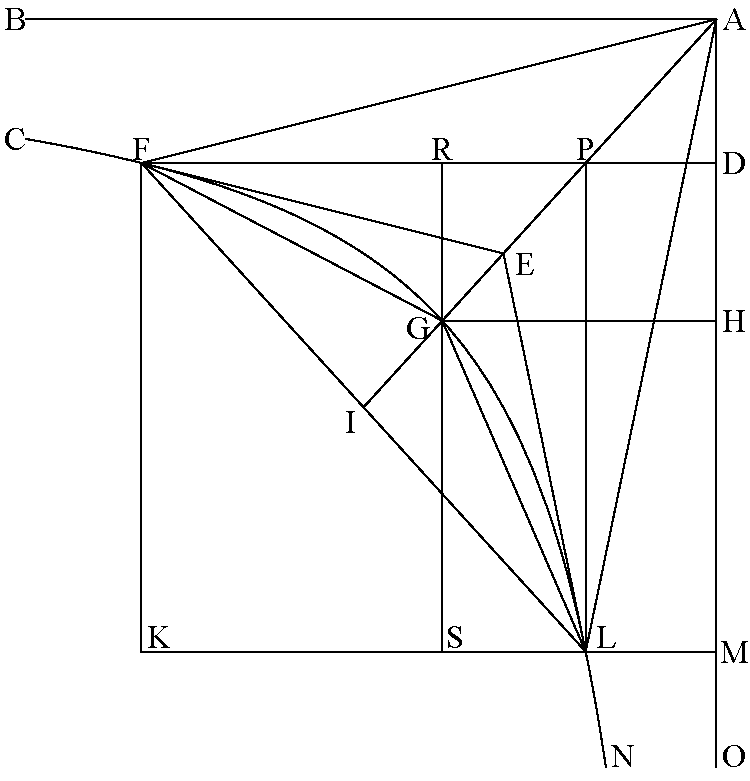
\includegraphics[scale=0.95]{vera_hyp_i}
\end{figure}

\begin{center}
\large\textsc{Proposition XXVII. Theorem.}
\end{center}

\vskip 1.0em
By the same assumptions, let line $AI$ be drawn bisecting $FL$ at $I$ and
intersecting the hyperbola at the point $G$. 
Also let $AFGL$ be a circumscribed quadrilateral of the sector. 
I claim that this is the geometric mean of parallelograms $FDMK$ and $PLMD$.
From the proof of Gregorie of St. Vincent it is evident that quadrilateral
$AFGL$ is equal to $DFGLM$. 
Because $AGI$ bisects the line $FL$ at $I$, from Gregorie of St. Vincent's Book
of the Hyperbola it is clear that the lines $LM$, $GH$, and $FD$ are
continually proportional in the same ratio with the three continuous
proportionals $AD$, $AH$, and $AM$. 
Let the line $RGS$ be drawn through the point $G$ parallel to the asymptote
$AO$, meeting the lines $FD$ and $MK$ at the points $R$ and $S$. 
Because the lines $FD$, $GH$, and $LM$ are continuously propotional, by dividing
and permuting we obtain $FR$ is to $SL$ as $GH$ is to $LM$. 
Likewise, since the lines $MA$, $HA$, and $DA$ are continuously proportional, by
dividing and permuting we obtain $MH$ is to $HD$, that is $SG$ is to $GR$, as
$HA$ is to $DA$, or $GH$ is to $LM$. 
Thus $FR$ is to $SL$ as $SG$ it to $GR$, and when the angles $FRG$ and
$GLS$ are equal, on account of parallels $FR$ and $SL$ being equal, the
triangles $FRG$ and $GLS$ shall be equal. 
Therefore parallelogram $RDMS$ is equal to polygon $DFGLM$, or quadrilateral
$AFGL$. 
However, parallelogram $RDMS$ is the geometric mean of parallelograms $PDML$
and $FDMK$ since by having the same height, the bases $LM$, $SM$ and $KM$ are
continuously proportional. 
Therefore the quadrilateral $AFGL$ is the geometric mean of parallelograms
$PDML$ and $FDMK$, as was to be shown.

\begin{center}
\large\textsc{Proposition XXVIII. Theorem.}
\end{center}

\vskip 1.0em
By the same assumptions, let the lines $FE$ and $LE$ be drawn tangent to the
hyperbola at points $F$ and $L$ in order to complete the quadrilateral $AFEL$. 
I claim this is the harmonic mean of parallelograms $PDML$ and $FDMK$. 
Triangle $AFL$, quadrilateral $AFGL$, and the harmonic mean of parallelograms
$PDML$ and $FDMK$ are continuously proportional since triangle $AFL$ is the
arithmetic mean and quadrilateral $AFGL$ the geometric mean of these
parallelograms, as is clear from Proposition 13. 
However triangle $AFL$, quadrilateral $AFGL$ and quadrilateral $AFEL$ are
continuously proportional by Proposition 11. 
Therefore quadrilateral $AFEL$ is the harmonic mean of parallelograms $PDML$
and $FDMK$, as was to be shown.

\begin{samepage}
\begin{center}
\large\textsc{Proposition XXIX. Problem.}

\vskip 1.0em
\emph{To find a square equal to a given circle.}
\end{center}
\end{samepage}

Let the square circumscribed by the circle be $4\cdot 10^{15}$, then the
inscribed square is $2\cdot 10^{15}$, between which \seqsplit{2828427124746190}
is the octagonal geometric mean. 
Now let the harmonic mean be between the octagon inside the circle and the
square about it, which by trivial labor is found by dividing the double of the
area of the octagonal inside the circle, or the double of the rectangle of the
areas inside and about the circle, by the sum of the square and the octagon
within. 
Then I find \seqsplit{3313708498984760} to be the harmonic mean, the
circumscribed octagon. 
Continuing this convergent series of complex polygons where the midpoint of
the first term is the same in each convergent term is easy to do up
to the polygon of 16384 sides. 
Indeed the inscribed is \seqsplit{3141592576586860} and the circumscribed
\seqsplit{3141592692091258}. 
This is not considered the final term, since in division and root extraction we
always stray in some small part from the true value, which is closely
approximated by this last imperfect term. 
Now the approximation from the proofs of Propositions 20 and
21 is used and the terms thus found will determine the true measure of the
circle, letting the square of the diamter be $4\cdot 10^{15}$, the smaller
circle \seqsplit{3141592653589789}, and the larger \seqsplit{3141592653589792}.
Thus the true measure of the circle may no longer hide, as was to be shown. 
I set out the following series of polygons.

\vskip 1.0em
\begin{tabular}{ r p{129pt} p{129pt} }
      & Inside the circle & About the circle \\
4     & 2000000000000000 & 4000000000000000 \\
8     & 2828427124746190 & 3313708498984760 \\
16    & 3061467458920718 & 3182597878074527 \\
32    & 3121445152258051 & 3151724907429255 \\
64    & 3136548490545938 & 3144118385245904 \\
128   & 3140331156954752 & 3142223629942456 \\
256   & 3141277250932772 & 3141750369168965 \\
512   & 3141513801144299 & 3141632080703181 \\
1024  & 3141572940367090 & 3141602510256808 \\
2048  & 3141587725277158 & 3141595117749588 \\
4096  & 3141591421543029 & 3141593269613390 \\
8192  & 3141592345578073 & 3141592807595664 \\
16384 & 3141592576586860 & 3141592692091258
\end{tabular}

\vskip 1.0em
The circle lies between the following terms
\[3141592653589789 \qquad\qquad 3141592653589792\]
and in precisely the same way an equivalent polygon to
any circular or elliptic sector inscribed by a known triangle and
circumscribed by a quadrilateral is obtained.

\begin{samepage}
\begin{center}
\large\textsc{Proposition XXX. Problem.}

\vskip 1.0em
\emph{To find an arc from a given sine.}
\end{center}
\end{samepage}

Let $AE$ be the arc of the circle described about the center $B$. 
The radius of this arc is of course $AB$ and the sine is $AD$. 
We want to find which proportion the arc itself has to the entire
circumference of the circle. 
Let $AE$ be the chord of the arc and its half-tangents be $AC$ and $CE$. 
From the square of the radius $AB$ is produced the square of the sine $AD$, and
square of the cosine $BD$ remains, and thus $BD$ is given. 
Therefore the area of the triangle $ABD$ is given by the rectangle and likewise
the area of the triangle $ABE$ is given, namely the rectangle of the given sine
$AD$ and half of the radius $BE$. 
From this it is seen that the sum of the triangles $ABD$ and
$ABE$ is to the triangle $ABE$ as the double of the triangle $ABE$ is to the
quadrilateral $ABEC$, which is given by Proposition 5. 
From the given inscribed triangle $ABE$ and the circumscribed quadrilateral
$ABEC$, the sector $ABE$ itself may be found by the preceding proposition, which
to the given entire circle has the desired proportion of the arc $AE$ to the
total circumference, which was to be shown.

\begin{samepage}
\begin{center}
\large\textsc{Proposition XXXI. Problem.}

\vskip 1.0em
\emph{To find a sine from a given arc.}
\end{center}
\end{samepage}

\begin{figure}[h!]
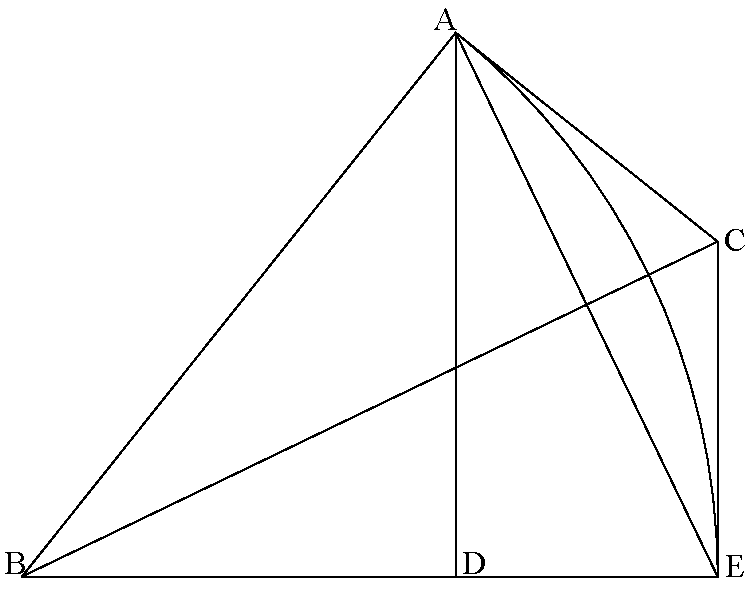
\includegraphics[scale=0.95]{vera_ii}
\end{figure}

From the given arc it is clear how to give the area of the sector. 
Therefore given the sector one may consider from how many arithmetic marks the
entire sine is made. 
Now part of such a given sector having been supposed, namely the
sector $ABE$, when the inscribed triangle $ABE$ and circumscribed quadrilateral
$ABEC$ are repeated as many times as desired, the given sector is a
multiple of the sector $ABE$ agreeing in every arithmetic term as the square
root of the whole sine contains. 
Indeed this can easily be shown from consideration of the table of
Proposition 29. 
Precision is not required in this process, for if large radii are
used then it makes no difference if the difference is off by a few parts. 
The radius $BA$ is given from the known sector $ABE$, by which the arc $AE$ is
likewise known. 
Let its sine $AD$ be given by $z$. 
Thus from the given sine and radius, the inscribed triangle $ABE$ is given as in
the previous proposition, as well as the circumscribed quadrilateral $ABEC$. 
And so the sector itself is given, it is the second of the two continuously
proportional arithmetic means of the inscribed triangle and the circumscribed
quadrilateral. 
Thus is given the equation between the double of the quadrilateral $ABEC$ plus
triangle $ABE$ and the triple of the known sector $ABE$, from whose resolution
the value of the unknown magnitude $z$ is obvious, which is the sine of $AD$. 
And by the given arc $AE$ and its sine likewise the sine of all of the
repetitions of the arc $AE$ is given from the common doctrine on the angle of a
sector. 
Therefore the sine of the proposed arc cannot hide, when it be in a
given multiple of the arc $AE$, which was to be shown.

\begin{samepage}
\begin{center}
\large\textsc{Proposition XXXII. Problem.}

\vskip 1.0em
\emph{To find a square equal to the hyperbolic area bound by a hyperbolic
curve, one asymptote, and two a lines parallel to the other asymptote, which
space is equal to the hyperbolic sector having for its base the same curve.}
\end{center}
\end{samepage}

\begin{figure}[h!]
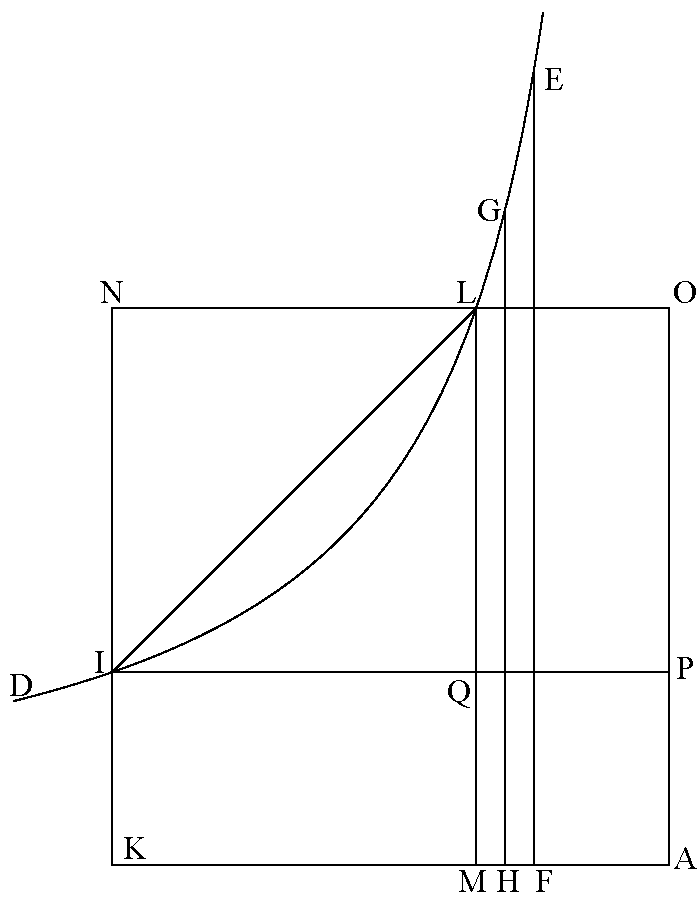
\includegraphics[scale=0.95]{vera_hyp_ii}
\end{figure}

Let $DIL$ be a hyperbola with asymptotes $AO$ and $AK$ that meet at the right
angle $OAK$. 
Consider the hyperbolic area $ILMK$ bounded by the hyperbolic
curve $IL$, the asymptotic segment $KM$, and the two lines $AK$ and $LM$, which
are parallel to the other asymptote $AO$. 
Choose the line $IK$ to be $10^{12}$, $LM$ to be $10^{13}$, and $AM$ to be
$10^{12}$ so that the line $KM$ is $9\cdot 10^{12}$. 
We want to find the measure of the area $ILMK$. 
Let the lines $IK$ and $OL$ be extended and draw the line $IP$ in order to
complete the rectangles $LNKM$ and $QIKM$. 
It is clear that rectangle $LNKM$ has area $9\cdot 10^{25}$ and $QIKM$ has area
$9\cdot 10^{24}$, and that the area of quadrilateral $LIKM$ is the arithmetic
mean of these rectangles, being $4.95\cdot 10^{25}$.
The geometric mean between $LNKM$ and $QIKM$ is found to
be \seqsplit{28460498941515413987990042} which is the regular circumscribed
pentagon of the hyperbolic area $LIKM$. 
Now as the quadrilateral $LIKM$ is to this circumscribed pentagon, so the double
of the pentagon is to the regular inscribed hexagon of the hyperbolic area
$LIKM$, namely \seqsplit{20779754131836628160009835}. 
This gives the complex of the regular hexagon with the aforementioned pentagon,
of which the two areas bring about the first terms of the convergent series.
Between this is the geometric mean by which the double of the square is divided
by the same geometric mean plus the greater term, or the circumscribed
pentagon. 
And they give the geometric mean and bear whatever proportion of the second
convergent terms. 
Thus this convergent series of complex polygons may be continued, while the
first midpoint of the terms is the same in both convergent terms, namely up to
the twentieth term, where the circumscribed polygon is
\seqsplit{2302585092993120329958961534173864} and the inscribed is
\seqsplit{23025850929931203593181124}. 
From here the approximation used is that proved in Propositions 23 and 24, and
the inscribed terms are discovered, describing the true hyperbolic area of
$LIKM$, being bound below by \seqsplit{23025850929940456240178681} and the same
area to be bound above by \seqsplit{23025850929940456240178704}. 
And so the area can no longer hide, which was to be shown. I thus deliver the
entire series of polygons plus the number of lines subtending the hyperbolic
curve in any circumscribed polygon.

\begin{landscape}
\begin{center}
{\renewcommand{\arraystretch}{0.8}
\begin{tabular}{ r p{190pt} p{180pt} }
        & Circumscribed Area         & Inscribed Area \\
2       & 28460498941515413987990042 & 20779754131836628160009835 \\
4       & 24318761696971474416609403 & 22410399968461612921314879 \\
8       & 23345088913234727934949897 & 22868197570682058351436953 \\
16      & 23105412906351426185065096 & 22986193244865462241217428 \\
32      & 23045725982658962868047234 & 23015921117139340153267671 \\
64      & 23030818728479610745741910 & 23023367512879647736902891 \\
128     & 23027092819292183214705676 & 23025230015404383009313933 \\
256     & 23026161398510805910921810 & 23025695697539046352276636 \\
512     & 23025928546847571901068394 & 23025812121604634087915779 \\
1024    & 23025870334152518169052273 & 23025841227841783762272302 \\
2048    & 23025855780992551911165543 & 23025848504414868310197241 \\
4096    & 23025852142703422669729927 & 23025850323559001769499206 \\
8192    & 23025851233131194254554390 & 23025850778345089029496888 \\
16384   & 23025851005738140519209367 & 23025850892041614212944994 \\
32768   & 23025850948889877295901163 & 23025850920465745719335070 \\
65536   & 23025850934677811503232115 & 23025850927571778609090592 \\
131072  & 23025850931124795055887228 & 23025850929348286832351848 \\
262144  & 23025850930236540944102405 & 23025850929792413888218560 \\
524288  & 23025850930014477416159412 & 23025850929903445652188450 \\
1048576 & 23025850929958961534173864 & 23025850929931203593181124 \\
\end{tabular}
}
\end{center}

\vskip 0.5em
\begin{center}
The hyperbolic sector lies between the following terms 

23025850929940456240178681 \qquad\qquad 23025850929940456240178704
\end{center}
\end{landscape}

It is therefore possible without danger of error to assume the following number
for the sector of the hyperbola, of which the multiples of the number up to ten,
facilitating division thanks to the composition of the logarithm, I reveal by
this.
For indeed in long division it is better to use repeated subtraction for
repetition of division than ordinary division, as any master of
arithmetic will agree.

It is clear that this problem can be resolved in the same way even if the
asymptotes $AO$ and $AK$ are not at a right angle. However we made assumptions
so that the problem would be easier and more readily used in the doctrine
of logarithms, which was first discovered by our most noble Napier, and which
we have now elevated (unless I am mistaken) to the highest peak of
perfection.

\begin{center}
\begin{tabular}{ r c }
1  & 23025850929940456240178700 \\
2  & 46051701859880912480357400 \\
3  & 69077552789821368720536100 \\
4  & 92103403719761824960714800 \\
5  & 115129254649702281200893500 \\
6  & 138155105579642737441072200 \\
7  & 161180956509583193681250900 \\
8  & 184206807439523649921429600 \\
9  & 207232658369454106161608300 \\
10 & 230258509299404562401787000 \\ [1.0em]
\end{tabular}
\end{center}


\begin{samepage}
\begin{center}
\large\textsc{Proposition XXXIII. Problem.}

\vskip 1.0em
\emph{To find the logarithm of any given number.}
\end{center}
\end{samepage}

\vskip 1.0em
By the same assumptions as in the preceding proposition, it is clear that,
taking $IK$ to be unity, $ML$ is ten. 
Therefore, $IK$ being unity, let $GH$ be any parallel to the asymptote $AO$,
then the logarithm of this given number is desired. 
It is clear from the given line $GH$ to get $KF$, and from the preceding
propositions how to get the hyperbolic area $GIKH$, and I claim that this
hyperbolic area the logarithm of the proposed number $GH$. 
I take by the area $LIKM$ the logarithm of the number ten. 
Indeed (from Gregorie of St. Vincent) the area $GHKI$ is in the same ratio to
the area $LMKI$, as the ratio $GH$ to $IK$ is a multiple of the ratio $LM$ to
$IK$. 
However the ratio $GH$ to $IK$ is a multiple of the ratio $LM$ to $IK$ in the
same ratio as the number $GH$ is a multiple of the number $LM$, since it is
contained itself in both ratios. 
Thus the area $GIKH$ is in the same ratio to the area $LIKM$, in which the
number $GH$ is a multiple of the number $LM$, and so (since by hypothesis the
area $LIKM$ is the logarithm of the number $LM$, or ten) the area $GIKH$ shall
be the logarithm of the proposed number $GH$, since this is the essential
property of logarithms, as they be among themselves in the same direct ratio,
in which they are one another multiplied by the same number. 
And the logarithm of ten is generally given as a one with some arbitrary number
of zeros. 
If this be done, the area $LIKM$ is to the area $GIKH$ as the arbitrary
logarith of ten is to the other number. 
That number shall be found to be the logarithm of the proposed
number $GH$, which we wanted to find.

\begin{center}
\large\textsc{Scholium.}
\end{center}

\vskip 1.0em
The exercise of the preceding set of problems is long and laborious. Thus in
order to abbreviate our labor when composing tables of logarithms, it has been
understood that we merely need to work on the discovery of logarithms of prime
numbers. Indeed the logarithms of composite numbers are found without effort
from the primes by addition and subtraction. However as the logarithms of prime
numbers may be easily found, the order progressing from the priors to the
latters, so that from the arbitrary logarithm of 10 to each prime number 2, and
from 10 and 2 to 3, likewise from 10, 2, and 3 to 7, likewise from 10, 2, 3, and
7 to 11, and thus hereafter. Next two composite numbers differing by very little
are found, of which one is composed from a number having a known logarithm, and
so having the given logarithm, the other number is composed from only a prime
number (of which the logarithm is found) or from that plus another number having
known logarithm. Now these composite numbers are drawn (which may be, e.g., $GH$
and $EF$) to the hyperbola as parallels to the asymptote $OA$, and the
hyperbolic area $EGHF$ is found according to Proposition 32, which is done
quickly from $GH$ and $EF$, which differ by very little. By assumption, the
logarithm of one of the numbers, e.g. $GH$, is given, and so the ratio of its
logarithm to the arbitrary logarithm of ten is given, which is the same (from
the proofs to this point) as the ratio of the hyperbolic area $GIKH$ to the
hyperbolic area $LIKM$. However the area LIKM is given by Proposition 32, and
so the area $IKHG$ is known, and with the given area $EGHF$ $EIKF$ is given.
Thus the logarithm of the composite number $EF$ is given. And when by assumption
the logarithms of every number composing the number $EF$ may be given, except
that prime number of which the logarithm is desired, that logarithm of the prime
number will be given, which we wanted to find. For example, Let it be proposed
to find the logarithm of the number two, supposing arbitrarily the logarithm of
the number ten, but given as one with 25 zeros, the two composite numbers,
differing by very little, are 1000 and 1024. The logarithm of the number 1000,
or the triple of the area found above as \seqsplit{23025850929940456240178700},
namely that area given by the arbitrary logarithm of the number ten.

\begin{landscape}
\begin{center}
{\renewcommand{\arraystretch}{0.8}
\begin{tabular}{ r p{190pt} p{180pt} }
        & Circumscribed Area         & Inscribed Area \\
2       & 237170824512628449899917 & 237162487062045867846886 \\
4       & 237166655750699903737556 & 237164571388o54419219371 \\
8       & 237165613567087322970403 & 237165092476425954356426 \\
16      & 237165353021613523599438 & 237165222748948181485250 \\
32      & 237165287885271907848389 & 237165255317105572320456 \\
64      & 237165271601188181041012 & 237165263459146597159038 \\
\end{tabular}
}
\end{center}

\vskip 0.5em
\begin{center}
The hyperbolic sector lies between the following terms 

237165266173160272103220 \qquad\qquad 237165266173160458453029
\end{center}

\vskip 0.5em
Let the four greatest of the continuously arithmetic
proportionals of \seqsplit{237165266173160421183067} be between these terms,
which hence shall be the true sector of the hyperbola in the proposed number of
the noted, since the first third of the noted is the same in both of the
convergent terms.
\end{landscape}

\noindent Let the logarithm of the number 1024 be unknown, it is composed from
only the prime number 2, namely it is multiplied ten times. These composite
numbers are drawn to the hyperbola, as has been said, letting $GH$ be 1000 and
$EF$ be 1024. But since $IK$ is \seqsplit{1000000000000}, $GH$ shall be
\seqsplit{1000000000000000} and $EF$ \seqsplit{1024000000000000}, and by
Proposition 32 the area $EGHF$ is found to be
\seqsplit{237165266173160421183067} (I give this convergent series for the
profit of the reader), or the logarithm of the number $1\frac{24}{1000}$ by the
proposed arbitrary logarithm of ten \seqsplit{23025850929940456240178700}. Next,
by the same assumed arbitrary logarithm of ten, the logarithm of the number 1000
is added, or the triple of the logarithm of ten, to the logarithm of the number
$1\frac{24}{1000}$, and will give the logarithm of the sum of the number 1024,
of which a tenth part will be the logarithm of the number two through the same
arbitrary logarithm of ten, or \seqsplit{6931471805599452914171917}. So it will
be that the logarithm of the number ten \seqsplit{23025850929940456240178700} is
to the logarithm of the number two corresponding to
\seqsplit{6931471805599452914171917} as the proposed arbitrary logarithm of the
number ten, or \seqsplit{10000000000000000000000000} is to the logarithm of the
sought number two \seqsplit{3010299956639811952405804}, which we wanted to
find\footnote{That is, $\log_10 \left(2\right) = \frac{\log \left(2\right)}{\log
\left(10\right)}$}.
By the same method the logarithm of three is found to be
\seqsplit{4771212547196624373502993}, etc.

In order to show these composite numbers, differing very little among
themselves, through one of the prime numbers, I present this table for each
prime number up to 100, as well as one rule for prime numbers between 100 and
1000 and another for prime numbers above 1000, which have all been contrived so
that the true logarithm of any prime number can be found by the corresponding
arbitrary logarithm of ten \seqsplit{10000000000000000000000000} by only one
multiplication, two divisions, and one square root extraction, as well as some
little effort.

\begin{longtable}{ c l }
\multirow{2}[2]{*}{\Huge 2}  & $1000 = 10^{3}$ \\
                          & $1024 = 2^{10}$ \\ [1.0em]
\multirow{2}[2]{*}{\Huge 3}  & $32805 = 5\cdot 6561 = 5\cdot 3^{8}$ \\
                          & $32768 = 2^{15}$ \\ [1.0em]
\multirow{2}[2]{*}{\Huge 7}  & $2400 = 3\cdot 32 = 3\cdot 2^{5}$ \\
                          & $2401 = 7^{4}$ \\ [1.0em]
\multirow{2}[2]{*}{\Huge 11} & $9800 = 2\cdot 49\cdot 100 = 2\cdot 7^{2}\cdot 10^{2}$ \\
                          & $9801 = 121\cdot 81 = 11^{2}\cdot 3^{4}$ \\ [1.0em]
\multirow{2}[2]{*}{\Huge 13} & $123200 = 7\cdot 11\cdot 25\cdot 64 = 7\cdot 11\cdot 5^{2}\cdot 2^{6}$ \\
                          & $123201 = 169\cdot 729 = 13^{2}\cdot 3^{6}$ \\ [1.0em]
\multirow{2}[2]{*}{\Huge 17} & $2600 = 13\cdot 8\cdot 25 = 13\cdot 2^{3}\cdot 5^{2}$ \\
                          & $2601 = 9\cdot 289 = 3^{2}\cdot 17^{2}$ \\ [1.0em]
\multirow{2}[2]{*}{\Huge 19} & $28899 = 169\cdot 9\cdot 19 = 13^{2}\cdot 3^{2}\cdot 19$ \\
                          & $28900 = 100\cdot 289 = 10^{2}\cdot 17^{2}$ \\ [1.0em]
\multirow{2}[2]{*}{\Huge 23} & $25920 = 10\cdot 32\cdot 81 = 10\cdot 2^{5}\cdot 3^{2}$ \\
                          & $25921 = 49\cdot 529 = 7^{2}\cdot 23^{2}$ \\ [1.0em]
\multirow{2}[2]{*}{\Huge 29} & $613088 = 17\cdot 23\cdot 32\cdot 49 = 17\cdot 23\cdot 2^{5}\cdot 7^{2}$ \\
                          & $613089 = 729\cdot 841 = 3^{6}\cdot 29^{2}$ \\ [1.0em]
\multirow{2}[2]{*}{\Huge 31} & $116280 = 10\cdot 17\cdot 19\cdot 4\cdot 9 = 10\cdot 17\cdot 19\cdot 2^{2}\cdot 3^{2}$ \\
                          & $116281 = 121\cdot 961 = 11^{2}\cdot 31^{2}$ \\ [1.0em]
\multirow{2}[2]{*}{\Huge 37} & $165648 = 3\cdot 7\cdot 17\cdot 29\cdot 16 = 3\cdot 7\cdot 17\cdot 29\cdot 2^{4}$ \\
                          & $165649 = 121\cdot 1369 = 11^{2}\cdot 37^{2}$ \\ [1.0em]
\multirow{2}[2]{*}{\Huge 41} & $1413720 = 7\cdot 10\cdot 11\cdot 17\cdot 4\cdot 27 = 7\cdot 10\cdot 11\cdot 17\cdot 2^{2}\cdot 3^{3}$ \\
                          & $1413721 = 1681\cdot 841 = 41^{2}\cdot 29^{2}$ \\ [1.0em]
\multirow{2}[2]{*}{\Huge 43} & $978120 = 10\cdot 11\cdot 13\cdot 19\cdot 4\cdot 9 = 10\cdot 11\cdot 13\cdot 19\cdot 2^{2}\cdot 3^{2}$ \\
                          & $978121 = 529\cdot 1849 = 23^{2}\cdot 43^{2}$ \\ [1.0em]
\multirow{2}[2]{*}{\Huge 53} & $664848 = 7\cdot 19\cdot 23\cdot 8\cdot 125 = 7\cdot 19\cdot 23\cdot 2^{3}\cdot 5^{3}$ \\
                          & $664849 = 9\cdot 121\cdot 2809 = 3^{2}\cdot 11^{2}\cdot 53^{2}$ \\ [1.0em]
\multirow{2}[2]{*}{\Huge 57} & $5851560 = 3\cdot 5\cdot 13\cdot 31\cdot 121 = 3\cdot 5\cdot 13\cdot 31\cdot 11^{2}$ \\
                          & $5851561 = 1681\cdot 3481 = 41^{2}\cdot 57^{2}$ \\ [1.0em]
\multirow{2}[2]{*}{\Huge 61} & $3575880 = 5\cdot 7\cdot 11\cdot 43\cdot 8\cdot 27\cdot = 5\cdot 7\cdot 11\cdot 43\cdot 2^{3}\cdot 3^{3}$ \\
                          & $3575881 = 961\cdot 3721 = 31^{2}\cdot 61^{2}$ \\ [1.0em]
\multirow{2}[2]{*}{\Huge 67} & $1620528 = 3\cdot 13\cdot 16\cdot 49 = 3\cdot 13\cdot 2^{4}\cdot 7^{2}$ \\
                          & $1620529 = 361\cdot 4489 = 19^{2}\cdot 67^{2}$ \\ [1.0em]
\multirow{2}[2]{*}{\Huge 71} & $2016399 = 3\cdot 11\cdot 29\cdot 43\cdot 49 = 3\cdot 11\cdot 29\cdot 43\cdot 7^{2}$ \\
                          & $2016400 = 16\cdot 25\cdot 5041 = 2^{4}\cdot 5^{2}\cdot 71^{2}$ \\ [1.0em]
\multirow{2}[2]{*}{\Huge 73} & $5116644 = 4\cdot 9\cdot 169\cdot 841 = 2^{2}\cdot 3^{2}\cdot 13^{2}\cdot 29^{2}$ \\
                          & $5116645 = 7\cdot 17\cdot 19\cdot 31\cdot 73$ \\ [1.0em]
\multirow{2}[2]{*}{\Huge 79} & $5997600 = 17\cdot 32\cdot 9\cdot 25\cdot 49 = 17\cdot 2^{5}\cdot 3^{2}\cdot 5^{2}\cdot 7^{2}$ \\
                          & $5997601 = 961\cdot 6241 = 31^{2}\cdot 79^{2}$ \\ [1.0em]
\multirow{2}[2]{*}{\Huge 83} & $1164240 = 5\cdot 11\cdot 16\cdot 27\cdot 49 = 5\cdot 11\cdot 2^{4}\cdot 3^{3}\cdot 7^{2}$ \\
                          & $1164241 = 169\cdot 6889 = 13^{2}\cdot 83^{2}$ \\ [1.0em]
\multirow{2}[2]{*}{\Huge 89} & $2859480 = 5\cdot 47\cdot 8\cdot 9\cdot 169\cdot = 5\cdot 47\cdot 2^{3}\cdot 3^{2}\cdot 13^{2}$ \\
                          & $2859481 = 361\cdot 7921 = 19^{2}\cdot 89^{2}$ \\ [1.0em]
\multirow{2}[2]{*}{\Huge 97} & $1138488 = 3\cdot 13\cdot 41\cdot 89\cdot 8 = 3\cdot 13\cdot 41\cdot 89\cdot 2^{3}$ \\
                          & $1138489 = 121\cdot 9409 = 11^{2}\cdot 97^{2}$ \\ [1.0em]
\end{longtable}

For prime numbers between 100 and 1000 let this be the rule: before the prime
number of which the logarithm is desired, the two numbers immediately preceding
are assumed, and the number following immediately after it, which three numbers
with that prime are four numbers following one after another in natural order
among themselves. Next the first number is multiplied by the cube of the third
and the fourth by the cube of the second, and it will be that their difference
equals the sum of the prime and the fourth or of the second and the third, as
can easily be shown. These numbers have at least six prime factors between them,
and thus they differ very little among themselves. Also the logarithms of the
four of these numbers (except the third) are known from the preceding method,
and thus are suitable to our abbreviation. So much apparatus is not useful in
numbers beyond 1000, since the rectangle of the numbers, among which the prime
number is understood immediately of which the logarithm is desired, which is
only less the square of the prime number by one. And so these have at least six
prime factors among them, and the logarithms of the first and third are
obtained. Therefore the infinitude are available to us.

\begin{samepage}
\begin{center}
\large\textsc{Proposition XXXIV. Problem.}

\vskip 1.0em
\emph{From a given logarithm to find its number.}
\end{center}
\end{samepage}

\vskip 1.0em
From the demonstration it is clear that this problem is the same as that which
was proposed, namely from the given hyperbolic area and one line understood to
be parallel to one of the asymptotes, to find another area and its parallel to
the asymptote. It may be considered from however many arithmetic terms comprise
the arbitrary logarithm of ten, and the logarithms or
the given area, the area $LIKM$, being assumed so that the regular
circumscribed polygons of the area $LIKM$ and the regular inscribed hexagons of
the same be repeated however many times, the given area being repeated
to the area $LIKM$, agreeing in all arithmetic terms, as many the square root
of the arbitrary logarithm of ten contains. Indeed this can be done easily from
the table of Proposition 32. Therefore the measure of the area $LIKM$ is
obtained and the line $IK$ is unity by assumption. Let $LM$ be $z$. As in
Proposition 32 the regular circumscribed pentagon and the regular inscribed
hexagon give the area $LIKM$, between which the given area $LIKM$ is the
second of the two continuously proportional arithmetic means. And so the double
of the hexagon plus the pentagon is equal to the triple of the area, which
equation the unknown $z$, or the number $LM$, clearly resolves, which
repeated however many times, as many as the area $LIKM$ is submultiplied to the
space, or the given logarithm, is the desired number, which was to be shown.

This is the same problem as Proposition 8, but more general and the method of
this solution is far less work.

\begin{samepage}
\begin{center}
\large\textsc{Proposition XXXV. Problem.}

\vskip 1.0em
\emph{A line having been drawn through a given point on a diamter, to divide
the semicircle into a given ratio.}
\end{center}
\end{samepage}

\begin{figure}[h]
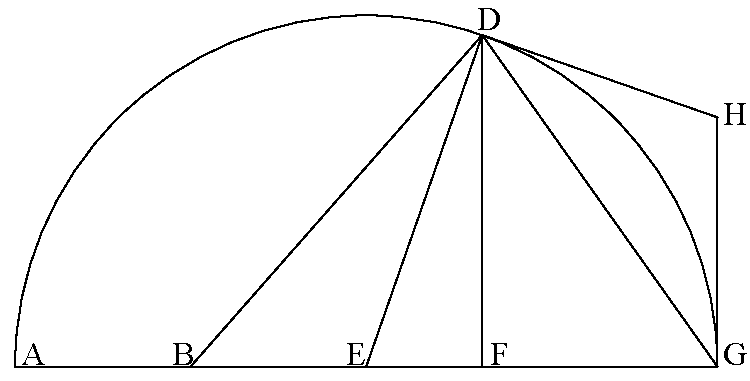
\includegraphics[scale=0.95]{vera_semicirc}
\end{figure}

\vskip 1.0em
Let $ADG$ be a semicircle of given diameter $AG$, center $E$, and $B$ be a given
point on the diameter. Assume it is made as described, and let the line $BD$
divide the semicircle into a given ratio. Since the measure of the semicircle is
given and the ratio into which it is divided, its portion, $DBG$, is given.
Let $z$ be the line $BD$. From the given lines $BD$, $BE$, and $ED$, the
triangles $DEB$, $DEF$, and $DEG$ are known. Next let it be that as $DEF$
plus $DEG$ is to $DEG$ so the double of $DEG$ is to the circumscribed
quadrilateral $DEGH$. Setting $DEG$ and $DEGH$ as the first convergent term, the
convergent series of complex ploygons may be continued, repeated as often as
necessary according to the properties of the circle until the agreed upon
approximation is met so that the sector $DEG$ is reached, which itself plus the
triangle $DBE$ is euqal to the known value $DBG$, the equation of which
is clearly resolved by the unknown magnitude $z$, or the line $BD$. The rest is
obvious.

The same problem is resolved in precisely the same way in the ellipse, the
hyperbola, or any sector given.

\begin{center}
\large\textsc{Scholium.}
\end{center}

\vskip 1.0em
If a set of problems for the previous Propositions is desired for mechanical
pratice, it will not be difficult to imitate the calculation, approximation, and 
resolution of equations to some extent according to the common rules of the
practice of Geometry. Many such problem sets may be resolved by the power of
analysis and by our rules of convergent series, which before may have been
impossible to estimate. However, it will be strongly claimed by many that
these solutions are not geometric. I respond that if the only practice
understood by the geometer is the power of the straightedge and compass, not
only will this be impossible but likewise will every problem set which cannot
be reduced to a quadratic equation, as may easily be shown. And if the
reduction of the problem to an analytic equation be understood by the geometer,
all of this problem set are impossible to the geometer, where by this proof it
is clear that such a reduction is cannot be done. If in truth this most simple
method of every possibility be understood by the geometer, it will be found
most strongly after timely consideration that the entirety of the above problem
set may be resolved most geometrically. Carefully observing the whole doctrine
of convergent series it is possible likewise by little effort to apply it to simple series. Indeed
let $A$, $B$, $C$, $D$, $E$, etc. be a series of such nature that the third term
$C$ is composed by the same method from the first and second terms $A$ and $B$
as the fourth term $D$ is composed from the second and third terms $B$ and $C$,
and the fifth $E$ from the third and fourth $C$ and $D$, and so on infinitely.
Let also the difference of the aforementioned $A$ and$B$ be always greater than
the difference of the subsequent terms $B$ and $C$. We may assume this series to
continue infinitely until two of the adjacent terms are not different, and
letting one of these terms be $z$, which we call the limit of the series. I
claim that $z$ is composed by the same method from $A$ and $B$ as from $B$ and
$C$ or $C$ and $D$. The proof scarcely differes from that of Proposition 10 and
its Conclusions. If this ratio is put to a triangle, inscribed in a sector of a
circle or ellipse or circumscribed to a sector of a hyperbola, $a$, and a
quadrilateral, regularly inscribed in a circle or ellipse or circumscribed to a
hyperbola, $b$, then the hexagon regularly inscribed in a sector of a circle or
ellipse or circumscribed to a hyperbola will be $\sqrt{\frac{2b^{3}}{a+b}}$.
Thus the sector of a circle, ellipse, or hyperbola is composed of the same method
from $a$ and $b$ as from $b$ and $\sqrt{\frac{2b^{3}}{a+b}}$. And so this
likewise can be shown, that the ratio of the sector to its given triangle may not be
analytic, according to Proposition 11. It would actually be possible to yet
prove by another particular method that the circular arc does not have an
analytic ratio to its given chord, but I do not add more, meanwhile advising
geometers to growth by science. I myself might have discovered in certain
figures (which Descartes called the second type) three foci, or three points,
from which lines drawn to any point of the curve the sum or difference is always
the same. Whence it appears to me to be true as all curves of the first type
have two foci whether real or imaginary, as all of the second type have three,
all third four, and so on infinitely. This speculation is certainly most worthy
of scrutiny, and indeed it may be an extraordinary property of the geometric
figures, and of the most useful mechanical practice of all equations.

\begin{center}
\Huge FINIS.

\vskip 0.5em
Anno Dom: 1667.
\end{center}
\iffalse
\cleardoublepage
\appendix
\begin{center}
\LARGE\textsc{Appendix.} \\
\large\emph{A modern rendering of the propositions.}
\end{center}

\vskip 2.0em

\begin{center}
Proposition I:
\end{center}
Let the area of $BAPF=a$, the area of $BAP=b$, and the area of $BAPI = c$. Then
$c = \frac{a + b}{2} = \textrm{AM} \left( a, b \right)$.

\vskip 2.0em
\begin{center}
Proposition II:
\end{center}
Let the area of $AFBP = a$, the area of $ABIP = b$, and the area of $ABDLP = c$.
Then $c = \frac{2ab}{a+b} = \frac{\textrm{GM} \left( a, b \right)}{\textrm{AM}
\left( a, b \right)}$.

\vskip 2.0em
\begin{center}
Proposition III:
\end{center}
Let the area of $ABIP = a$, the area of $BAP = b$, and the area of $ABDLP = c$.
Then $c = \frac{2a^2}{a+b} = \frac{a^2}{\textrm{AM} \left( a, b \right)}$.

\vskip 2.0em
\begin{center}
Proposition IV:
\end{center}
Let the area of $ABIP = a$, the area of $ABDLP = b$, and the area of $ABEIOP =
c$. Then $c = \frac{a + b}{2} = \textrm{AM} \left( a, b \right)$.

\vskip 2.0em
\begin{center}
Proposition V:
\end{center}
Let the area of $ABEIOP = a$, the area of $ABIP = b$, and the area of polygon
$ABCGKNP = c$. Then $c = \frac{2a^2}{a+b} = \frac{a^2}{\textrm{AM} \left( a, b
\right)}$.

\vskip 2.0em
\begin{center}
Proposition VI:
\end{center}
Let the area $ABP = a$, the area of $ABFP = b$, the area of $ABIP = c$, and the
area of $ABDLP = d$. Then $a - b \leq 2\left( c - d \right) = \frac{(a + b)^2}{a
+ 3b} = \frac{2\textrm{AM}^2 \left( a, b \right)}{\textrm{AM} \left( a, b
\right) + b}$.

\vskip 2.0em
\begin{center}
Proposition VII:
\end{center}
Let $a_{0} = a$ and $b_{0} = b$ where $a < b$ and 
\fi

\bibliographystyle{plain}
\bibliography{cite1}
\end{document}















